\documentclass[11pt]{article}
\usepackage[margin=1in]{geometry}
\usepackage{amsmath,amssymb,amsthm,mathtools,bm}
\usepackage{booktabs,graphicx,float,caption,subcaption,array,multirow}
\usepackage[authoryear,round]{natbib}
\usepackage[hidelinks]{hyperref}
\usepackage{parskip}
\usepackage{enumitem}
\setlist{itemsep=2pt,topsep=4pt}

\graphicspath{{../results/}}
\captionsetup{font=small,labelfont=bf}

\theoremstyle{plain}
\newtheorem{proposition}{Proposition}[section]
\newtheorem{lemma}[proposition]{Lemma}
\newtheorem{corollary}[proposition]{Corollary}
\newtheorem{theorem}[proposition]{Theorem}
\theoremstyle{definition}
\newtheorem{definition}[proposition]{Definition}
\newtheorem{assumption}[proposition]{Assumption}
\theoremstyle{remark}
\newtheorem{remark}[proposition]{Remark}

\newcommand{\E}{\mathbb{E}}
\newcommand{\Q}{\mathbb{Q}}
\newcommand{\Prob}{\mathbb{P}}
\newcommand{\1}{\mathbf{1}}
\newcommand{\ctrig}{c_{\mathrm{trig}}}
\newcommand{\cmda}{\bar c}
\newcommand{\lres}{\lambda_{\mathrm{res}}}
\newcommand{\lspec}{\lambda_{\mathrm{spec}}}
\newcommand{\G}{\mathcal{G}}
\newcommand{\F}{\mathcal{F}}
\newcommand{\dd}{\,\mathrm{d}}

\title{\textbf{Pricing Additional Tier~1 Bonds as Claims on Bank Capital}\\[6pt]
\large A capital-ratio model with a stochastic refinancing spread, a Tier~2 anchor\\
for the write-down hazard, and an application to BNP Paribas}
\author{Paolo Mastrogiacomo\thanks{Credit-Quant-Research, \texttt{at1-coco-pricer}.
Code, tests and the scripts that produce every number and figure in this paper are in the
repository. Market data are S\&P Capital IQ evaluated prices and are not redistributed.
Academic work, not investment advice.}}
\date{October 2026}

\begin{document}
\maketitle

\begin{abstract}
\noindent
Additional Tier~1 (AT1) bonds are perpetual, deeply subordinated bank bonds whose
coupons, principal and redemption all depend on the issuer's capital. We model them
as claims on the Common Equity Tier~1 (CET1) ratio, which follows a mean-reverting
jump-diffusion, together with a correlated stochastic refinancing spread that drives
both the issuer's call decision and a doubly-stochastic write-down hazard. Coupons are
restricted by the Maximum Distributable Amount (MDA) rule along a time-varying
regulatory threshold, principal converts at a contractual trigger, and the issuer calls
only when refinancing is cheaper. Conditioning on the state paths makes the price an
explicit, smooth, strictly decreasing and convex function of the hazard level, so the
market-implied hazard is unique, is solved without simulation noise in the hazard
direction, and every comparative static is computed with common random numbers.
We then price the issuer's Tier~2 and senior non-preferred bonds on the same simulated
state. Because the creditor hierarchy makes Tier~2 exposed to the same resolution event
as AT1, this splits the AT1 hazard into a part that Tier~2 also prices and an
AT1-specific premium. Calibrated to BNP Paribas's three USD AT1s on 25 September 2026,
the bonds imply a hazard of $2.19\%$ a year, equal across bonds to within the
bid--offer, of which $1.72\%$ is priced in BNP's Tier~2. Of the $\approx 275$bp spread,
about $180$bp is priced in Tier~2 as well, a figure that is robust to a reputational call
rule, to the order of attribution, to a term structure of the resolution hazard and to
the dynamics of capital. The remaining $90$--$100$bp, equally robust, pays for being an
AT1 rather than a Tier~2: MDA coupon cuts, conversion, extension and an AT1-specific
premium. How it divides among them depends on how fast the bank rebuilds capital, which
history identifies poorly: the premium is about $50$bp in the base case and zero at the
historical estimate, where coupon cuts and extension take its place. The Tier~2 restricts this dependence,
because pricing the AT1 as safer than the Tier~2 would violate the creditor hierarchy;
the restriction rules out the slower half of the plausible range of capital mean
reversion. Prices are flat in capital above the MDA threshold and steep at it, so the
risk-relevant distance is to the MDA threshold, not to the trigger.

\medskip\noindent
\textbf{Keywords:} contingent convertibles, AT1, CoCos, bank capital, MDA, point of
non-viability, Cox processes, conditional Monte Carlo, Shapley value.\\
\textbf{JEL:} G12, G13, G21, G28.
\end{abstract}

\newpage
\tableofcontents
\newpage

%======================================================================
\section{Introduction}\label{sec:intro}
%======================================================================

Additional Tier~1 (AT1) bonds, often called contingent convertibles or CoCos, are the
most equity-like instruments that European banks issue as debt. They count as
going-concern Tier~1 capital under the Capital Requirements Regulation, they are
perpetual and callable only by the issuer, their coupons are fully discretionary and
non-cumulative, and their principal is converted into shares or written down when the
bank's Common Equity Tier~1 (CET1) ratio falls below a contractual trigger. In
addition, the resolution authority can impose losses on them at the point of
non-viability (PONV), whatever the level of the trigger. The write-down of
CHF~16 billion of Credit Suisse AT1s in March 2023, while the bank reported a CET1
ratio around $14\%$, made the last feature the dominant one in market pricing.

Every one of these cash-flow contingencies is written, directly or indirectly, on the
bank's capital. The trigger is a CET1 level; the coupon restriction of the Maximum
Distributable Amount (MDA) regime is triggered when CET1 falls inside the combined
buffer requirement; regulatory approval of a call requires the bank to remain above its
requirements after redemption; and the regulator's decision to declare the bank
failing or likely to fail is, in practice, informed by the same deterioration of
capital and market access. This paper takes that observation literally: it models the
AT1 bond as a claim on the CET1 ratio, rather than as a straight bond with an equity
barrier attached.

\paragraph{Why not an equity barrier.}
The workhorse market model for CoCos treats conversion as a barrier event on the share
price \citep{DeSpiegeleerSchoutens2012}. That approach is convenient, because the share
price is observed and its volatility is quoted, but it needs a mapping from the share
price to the accounting ratio on which the contract is written. That mapping is not
observable and not stable: banks' equity traded at a fraction of book value in 2023
with unchanged capital ratios, and at a premium in other periods. A model written on
the CET1 ratio makes the trigger, the MDA restriction and the call constraint
consistent by construction. Its cost is that CET1 is not traded and is observed
quarterly with a lag, so its dynamics must be estimated under the physical measure and
the residual risk premia must be absorbed elsewhere. We absorb them in a write-down
hazard that is implied from bond prices, and we then ask how much of that hazard the
bank's other bonds also price.

\paragraph{Capital alone is not enough.}
A model in which CET1 is the only state variable cannot price BNP Paribas's AT1s. With
the historical volatility of BNP's CET1 ratio, the trigger is $7.8$ percentage points
away and is almost never reached in simulation: the bonds would be worth $114$--$118$
against market prices of $94$--$98$. The call decision, moreover, depends on the cost
of refinancing in the market, which moves with sector spreads and not only with the
bank's capital. We therefore add a second state variable: the issuer's new-issue AT1
spread, a mean-reverting Gaussian process correlated with capital shocks, with a
capital add-on once CET1 enters the buffer. This spread does two jobs. It drives the
call decision, so that the issuer extends exactly when refinancing is expensive, and it
scales a doubly-stochastic write-down hazard, so that extension states are also the
states in which the bond is riskier. Without the second link, extension would be valued
with a discount rate that does not reflect the state, and the option not to call could
even look valuable to the investor; we show this explicitly in
Section~\ref{sec:robust}.

\paragraph{What the hazard prices.}
The implied write-down hazard absorbs everything the mechanical features leave
unexplained, and on its own it cannot tell the bank's credit risk apart from risk that is
specific to the instrument. The bank's other bonds can. Under the EU resolution
framework the creditor hierarchy is respected: CET1 absorbs losses first, then AT1, then
Tier~2. The joint statement of the Single Resolution Board, the EBA and ECB Banking
Supervision of 20 March 2023 reaffirmed this ordering after the Credit Suisse case.
Tier~2 bonds are therefore exposed to the same resolution event as AT1, at a better
recovery, but have none of the AT1's coupon discretion, MDA restriction, trigger or
perpetual extension. Pricing them on the same simulated state identifies how much of the
AT1 hazard is compensation that Tier~2 also earns.

\subsection{Contributions}

The paper makes five contributions.
\begin{enumerate}
  \item \textbf{A capital-ratio model with an endogenous call and a state-dependent
  hazard.} The CET1 ratio follows a mean-reverting jump-diffusion around the bank's
  target, the refinancing spread a correlated Ornstein--Uhlenbeck process, and the
  write-down time is a Cox process whose intensity is proportional to the effective
  spread. The MDA threshold is time-varying, which matters because scheduled buffer
  step-ups shrink the bank's cushion at constant capital.
  \item \textbf{An exact conditional Monte Carlo for the hazard.} Conditioning on the
  state paths integrates the write-down time out analytically. The price becomes an
  explicit function $V(\lambda)$ that is smooth, strictly decreasing and strictly convex,
  so the implied hazard is unique and is found by a bracketing root-finder on a single
  set of paths. The same construction prices Tier~2 bonds with a recovery leg and a
  piecewise term structure of the hazard.
  \item \textbf{A Tier~2 anchor for the AT1 hazard.} Writing the AT1 hazard as
  $\lambda=\lres+\lspec$, with two independent exponential clocks, gives the AT1 and the
  Tier~2 the right joint survival structure. Calibrating $\lres$ to the bank's Tier~2 and
  checking it against the senior non-preferred bond turns an unexplained premium into an
  observable part and an AT1-specific residual.
  \item \textbf{An order-robust attribution of the spread.} Sequential decompositions of
  a credit spread into its components depend on the order in which features are switched
  on. We compute the exact Shapley value over all orders and a Shapley value within
  blocks, and show which conclusions survive. The order matters for the extension
  component and not for the split between Tier~2-priced and AT1-specific risk.
  \item \textbf{An application with honest identification.} We calibrate the model to
  BNP Paribas's three USD AT1s, two Tier~2 bonds, one senior non-preferred bond and its
  senior CDS, with 50 quarters of CET1 history. We report Monte Carlo errors, price the
  identification limits of evaluated bid--offer quotes, bootstrap the capital dynamics
  and show which results depend on the weakly identified speed of capital mean
  reversion.
\end{enumerate}

\subsection{Main findings}

On 25 September 2026 the three AT1s trade at yield-to-call spreads of $269$--$280$bp
over call-matched Treasuries. The model reprices them with hazards of $2.21\%$,
$2.18\%$ and $2.19\%$ a year. The dispersion of $2.6$bp of hazard is about four
Monte Carlo standard errors but only $0.20$--$0.22$ points of price, the size of the
bid--offer: the bonds are consistent with a single hazard within the precision of the
data, and cannot discriminate between model variants that differ by a few basis points.

BNP's Tier~2 2035NC34 implies a resolution hazard of $1.72\%$ at the conventional
$20\%$ recovery, and the senior non-preferred bond $1.63\%$ at $40\%$: the two
instruments that share the resolution event agree under the Markit recovery
conventions, and the Tier~2 recovery that equalises them is $16\%$. The AT1 hazard
therefore splits into $1.72\%$ priced in Tier~2 and $0.47\%$ specific to the AT1. In
spread terms, about $180$bp of the AT1 spread is priced in Tier~2, $50$bp is an
AT1-specific premium, and $40$--$46$bp pays for the contract features: expected MDA
coupon cuts ($\approx30$bp, an upper bound), mechanical conversion ($\approx4$bp)
and extension ($6$--$15$bp, decreasing in the reset margin). Because the MDA component
is an upper bound and the total is fixed by the market price, the AT1-specific premium
is a lower bound.

The split survives three robustness checks. A reputational call rule raises the
probability of a call at the first reset from $49$--$58\%$ to $77$--$81\%$, close to
the levels practitioners quote, but moves neither the hazard nor its split. Every
attribution that prices the hazard before the contract features gives the same
$181/50$bp split. A two-piece resolution hazard bootstrapped from the two Tier~2 bonds
($1.40\%$ to 2030, $2.10\%$ after) changes the Tier~2-priced component by less than
5bp.

Capital risk is a cliff, not a slope. At BNP's $13\%$ CET1 ratio the price moves by
about $0.6$ points per point of capital; at the MDA threshold it moves by about four.
Crossing the threshold switches on three mechanisms at once: coupons are cut, the call
is blocked and the hazard rises. The distance that matters for risk management is the
distance to the MDA threshold, which the scheduled O-SII step-ups reduce from $2.5$ to
$2.0$ percentage points by 2028 at constant capital, not the distance to the trigger.
The level of the capital stress depends strongly on the speed of capital mean
reversion, which fifty quarters of history identify only to within a factor of eight;
across that interval the price impact of the EBA adverse scenario ranges from $-7$ to
$-38$ points.

\subsection{Related literature}

\paragraph{Contingent capital.} The academic literature on contingent capital starts
from structural models in which the trigger is written on the value of the bank's
assets or on an accounting ratio. \citet{Pennacchi2010} models bank assets as a
jump-diffusion and prices CoCos with a trigger on the ratio of equity to assets;
\citet{GlassermanNouri2012} derive closed-form prices for contingent capital with a
capital-ratio trigger and gradual conversion. \citet{Flannery2014} surveys the design
issues, including the choice between market and accounting triggers and the role of
regulatory discretion. These models are built to study incentives and design, and
typically do not include the MDA restriction, the issuer's call option or a regulatory
write-down hazard independent of the trigger. Market practice instead relies on
reduced-form or equity-barrier models \citep{DeSpiegeleerSchoutens2012}, in which the
trigger is approximated by a barrier on the share price. \citet{AvdjievEtAl2013}
describe the market and the instrument features in detail. Our model sits between the
two: the state is the accounting ratio on which the contract is written, as in the
structural tradition, but the regulatory and market features that dominate AT1 pricing
today (discretionary coupons, MDA, issuer calls, PONV) are modelled explicitly and the
residual risk is priced in reduced form.

\paragraph{Reduced-form credit risk.} The write-down time is a doubly-stochastic
(Cox) process in the sense of \citet{Lando1998}, with intensity driven by the state, as
in the reduced-form models of \citet{JarrowTurnbull1995} and \citet{DuffieSingleton1999};
\citet{BieleckiRutkowski2002} give the general construction. Our use of the
construction is specific in two respects. First, the intensity is proportional to the
issuer's simulated refinancing spread, which also drives the call, so that the hazard
and the extension decision are consistent state by state. Second, we split the
intensity into two independent clocks to price the AT1 and the Tier~2 jointly, which
is the reduced-form counterpart of the creditor hierarchy.

\paragraph{Monte Carlo methods.} Integrating the default time out conditionally on the
state paths is a form of conditional Monte Carlo, or Rao--Blackwellisation
\citep{Glasserman2004}; it removes the variance due to the default event and makes the
price smooth in the hazard. Discrete monitoring of the trigger introduces the usual
bias of barrier options, which \citet{BroadieGlassermanKou1997} correct with a shift of
the barrier; we show that the correction is negligible here.

\paragraph{Decomposition and attribution.} Attributing a spread to its components by
switching features on one at a time is order-dependent whenever the features interact.
The Shapley value \citep{Shapley1953} resolves the dependence by averaging over all
orders, and \citet{Shorrocks2013} applies it to decompositions in economics; the value
for games with a priori unions \citep{Owen1977} handles groups of related factors. We
use both ideas and show that, for AT1 bonds, the economically consistent attribution
prices the hazard before the contract features.

\subsection{Outline}

Section~\ref{sec:institutions} describes the instrument, the regulatory framework and
the three BNP Paribas bonds. Section~\ref{sec:model} sets out the model and derives
the properties of the state processes. Section~\ref{sec:valuation} derives the pricing
equations, the conditional Monte Carlo estimator and its properties, and the pricing of
Tier~2 and senior bonds. Section~\ref{sec:attribution} defines the spread attribution.
Section~\ref{sec:calibration} describes the data and the calibration.
Section~\ref{sec:results} reports the results, Section~\ref{sec:robust} the robustness
checks and Section~\ref{sec:discussion} discusses implications and limitations. The
appendices contain proofs, numerical diagnostics and the parameter table.

%======================================================================
\section{The instrument and the regulatory framework}\label{sec:institutions}
%======================================================================

This section describes the features of AT1 bonds that the model must reproduce, the
regulatory rules behind them, and the three BNP Paribas bonds studied in the paper.
References to articles are to the Capital Requirements Regulation (CRR, Regulation (EU)
No 575/2013), the Capital Requirements Directive (CRD, Directive 2013/36/EU) and the
Bank Recovery and Resolution Directive (BRRD, Directive 2014/59/EU), as amended.

\subsection{Place in the capital structure}

A bank's own funds are layered. Common Equity Tier~1 (CET1) is ordinary share capital
and reserves; Additional Tier~1 (AT1) instruments complete Tier~1 capital, the
going-concern layer; Tier~2 instruments are gone-concern capital, subordinated debt
with an original maturity of at least five years. Below own funds, the bank's
loss-absorbing capacity in resolution (TLAC for global systemically important banks,
MREL for all banks) is completed by senior non-preferred debt, which ranks ahead of
Tier~2 but behind senior preferred debt and deposits.

In a liquidation or a resolution the creditor hierarchy determines the order in which
losses are absorbed: CET1 first, then AT1, then Tier~2, then senior non-preferred, then
senior preferred. For pricing purposes this ordering has a precise implication that we
use in Section~\ref{sec:t2}: every resolution event that imposes losses on Tier~2 has
already wiped out the AT1, while the converse is not true. AT1 holders are exposed to
all resolution events and, in addition, to events that hit AT1 alone.

\subsection{Eligibility and the perpetual call structure}

To count as AT1, an instrument must be perpetual, with no incentive to redeem (CRR
Art.~52). The issuer may call it no earlier than five years after issuance, and only
with the prior permission of the competent authority (Art.~77). Permission requires
that the instrument be replaced by own funds of equal or higher quality on terms that
are sustainable for the bank's income, or that the bank demonstrate that its own funds
would exceed its requirements by a margin the authority considers necessary (Art.~78).

The bonds studied here are callable only on their reset dates, every five years from
the first call. If not called, the coupon resets to the prevailing five-year US
Treasury constant-maturity yield plus the margin fixed at issuance. The fixed margin is
the source of extension risk: the issuer calls when it can refinance at a lower spread,
and does not call when spreads have widened, which is when investors would most like
their money back. Because the margin is fixed and the reference rate floats, the
economic call decision compares the reset margin with the issuer's new-issue AT1 spread
over the same benchmark; the level of rates cancels.

In practice, European issuers have called AT1s at the first opportunity in almost all
cases, partly for reputational reasons: a bank that does not call signals that its
funding is expensive. The best-known exception, Banco Santander's decision in early 2019
not to call a euro AT1, was widely reported precisely because it was rare. The model's
base call rule is purely economic; Section~\ref{sec:robust} adds a reputational
tolerance.

\subsection{Discretionary coupons and the Maximum Distributable Amount}

AT1 coupons are fully discretionary and non-cumulative: the issuer may cancel any
coupon at any time, cancelled coupons are lost, and cancellation is not an event of
default (CRR Art.~52(1)(l)). Coupons can only be paid out of distributable items.

In addition, coupons are mechanically restricted when the bank breaches its combined
buffer requirement (CRD Art.~141). Let the CET1 requirement be the sum of the Pillar~1
minimum ($4.5\%$ of risk-weighted assets), the CET1 part of the Pillar~2 requirement and
the combined buffer requirement (capital conservation, countercyclical, systemic risk
and G-SII/O-SII buffers). A bank whose CET1 ratio falls below this total may distribute
(dividends, variable remuneration and AT1 coupons together) at most the Maximum
Distributable Amount, a fraction of its interim and year-end profits that depends on
where the ratio sits inside the combined buffer:
\begin{center}
\begin{tabular}{lc}
\toprule
Position of CET1 inside the combined buffer & Maximum distributable fraction of profits \\
\midrule
top quartile & 0.6 \\
second quartile & 0.4 \\
third quartile & 0.2 \\
bottom quartile & 0 \\
\bottomrule
\end{tabular}
\end{center}
Two features of the rule matter for modelling. First, the MDA caps \emph{all}
distributions together; a bank inside the buffer chooses how to allocate the amount, and
would normally cut dividends, buy-backs and variable pay before cutting AT1 coupons,
which are small relative to profits and whose cancellation is costly for market access.
Applying the quartile factor to the coupon itself, as our model does, therefore
overstates the expected coupon loss. Second, analogous restrictions apply when the bank
breaches its leverage-ratio buffer (L-MDA) or its MREL requirement (M-MDA); for some
banks these bind before the CET1-based MDA.

\subsection{Loss absorption: trigger and point of non-viability}

Each AT1 contains a mechanical trigger: if the issuer's CET1 ratio falls below a
contractual level (at least $5.125\%$, CRR Art.~54), the instrument is converted into
ordinary shares or written down, permanently or temporarily. The bonds studied here
convert into shares at the higher of the prevailing market price and a floor price set
at issuance, so that the conversion ratio is capped.

Independently of the trigger, the resolution authority must write down or convert
capital instruments when the bank reaches the point of non-viability (BRRD Art.~59):
when the institution is failing or likely to fail and no alternative measure would
prevent its failure, or when public support is required. The write-down follows the
creditor hierarchy (BRRD Art.~48): CET1 first, then AT1, then Tier~2. A PONV write-down
can therefore occur while the CET1 ratio is far above the trigger. The Credit Suisse
case of March 2023, decided under Swiss law, wrote AT1 holders down to zero while
shareholders retained value; the EU authorities' joint statement of 20 March 2023
stated that in the EU, losses would continue to be absorbed by CET1 first and AT1 only
after CET1 had been fully used.

For pricing, this means two things. First, the PONV event is the dominant risk for a
well-capitalised issuer: the trigger is far away, but the regulator's decision is not
tied to it. Second, in the EU the PONV event that hits AT1 is, in most scenarios, the
same event that hits Tier~2. AT1 holders lose everything, Tier~2 holders lose part of
their claim. The AT1-specific part of the risk is the probability that AT1 is written
down while Tier~2 is not, together with the risk premia that investors attach to the
equity-like features of the instrument.

\subsection{The BNP Paribas bonds}

BNP Paribas is a global systemically important bank headquartered in France, supervised
by the ECB and resolvable by the Single Resolution Board. Its CET1 ratio was $12.97\%$ at
30 June 2026 against a published CET1 requirement of $10.43\%$. The latest stack available
item by item, at 30 September 2025, consists of Pillar~1 ($4.5\%$), the CET1 part of
Pillar~2R ($1.14\%$), the capital conservation buffer ($2.5\%$), the G-SIB buffer
($1.5\%$), the countercyclical buffer ($0.73\%$) and the systemic-risk buffer ($0.14\%$),
which sum to the $10.51\%$ requirement published at that date. The model takes the
Pillar~1 and Pillar~2R floor of $5.64\%$ from that stack and sets the combined buffer so
that the total equals the latest published requirement, $10.43\%$, so that the $8$bp
difference is attributed to the buffers. Under the French O-SII framework the
bank's O-SII buffer rises by 25bp on 1 January 2027 and by a further 25bp on 1 January
2028, and the higher of the G-SIB and O-SII buffers applies; at constant capital these
step-ups reduce the cushion above the MDA threshold from $2.5$ to $2.0$ percentage
points.

Table~\ref{tab:bonds} lists the three USD AT1s and the three bonds used as the Tier~2
and senior anchor. The AT1s share the issuer, the trigger ($5.125\%$ of group CET1), the
loss-absorption mechanism (conversion into ordinary shares) and the reset reference
(five-year US Treasury CMT); they differ in coupon, first call date and reset margin.
The Tier~2 and senior non-preferred (SNP) notes are callable once, one year before
maturity or at a reset date, when they cease to count as Tier~2 or MREL; the market
prices these calls as certain. The Tier~2 2035NC34 is the anchor: its call in November
2034 falls inside the AT1 call window (December 2033 to April 2036).

\begin{table}[H]
\centering\small
\begin{tabular}{llccccc}
\toprule
Bond & ISIN (144A) & Rank & Coupon & Call & Maturity & Reset margin \\
\midrule
6.875\% NC33 & US05602XQR25 & AT1 & 6.875\% & 15-Dec-2033 & perpetual & UST5 + 285bp \\
7.20\% NC36 & US05602XQS08 & AT1 & 7.200\% & 17-Apr-2036 & perpetual & UST5 + 294bp \\
7.45\% NC35 & US05602XQQ42 & AT1 & 7.450\% & 27-Jun-2035 & perpetual & UST5 + 313bp \\
\midrule
T2 2035NC34 & US09659T2D24 & T2 & 5.906\% & 19-Nov-2034 & 19-Nov-2035 & SOFR + 192bp \\
T2 2035NC30 & US09659T2B67 & T2 & 2.588\% & 12-Aug-2030 & 12-Aug-2035 & UST5 + 205bp \\
SNP 2035NC34 & US09659W2X16 & SNP & 5.738\% & 20-Feb-2034 & 20-Feb-2035 & SOFR + 188bp \\
\bottomrule
\end{tabular}
\caption{Bonds used in the paper. AT1s: perpetual, callable on reset dates every five
years, trigger $5.125\%$ of group CET1, conversion into ordinary shares at the higher of
the market price and a floor (USD 61.12, 72.52 and 61.17 per share respectively). Tier~2
and SNP: single call, treated as certain. Sources: BNP Paribas term sheets and debt
issuance list.}
\label{tab:bonds}
\end{table}

Figure~\ref{fig:prices} shows the AT1 prices over the sample. The 7.45\% has traded
since June 2025, the 6.875\% since December 2025 and the 7.20\% since April 2026. All
three fell by six to seven points over 2026, most of it from rising Treasury yields;
in the four weeks to 25 September 2026 the ten-year Treasury rose 45bp and the spread of
the low-margin 6.875\% widened by a further 34bp, against 10--12bp for the other two.

\begin{figure}[H]
\centering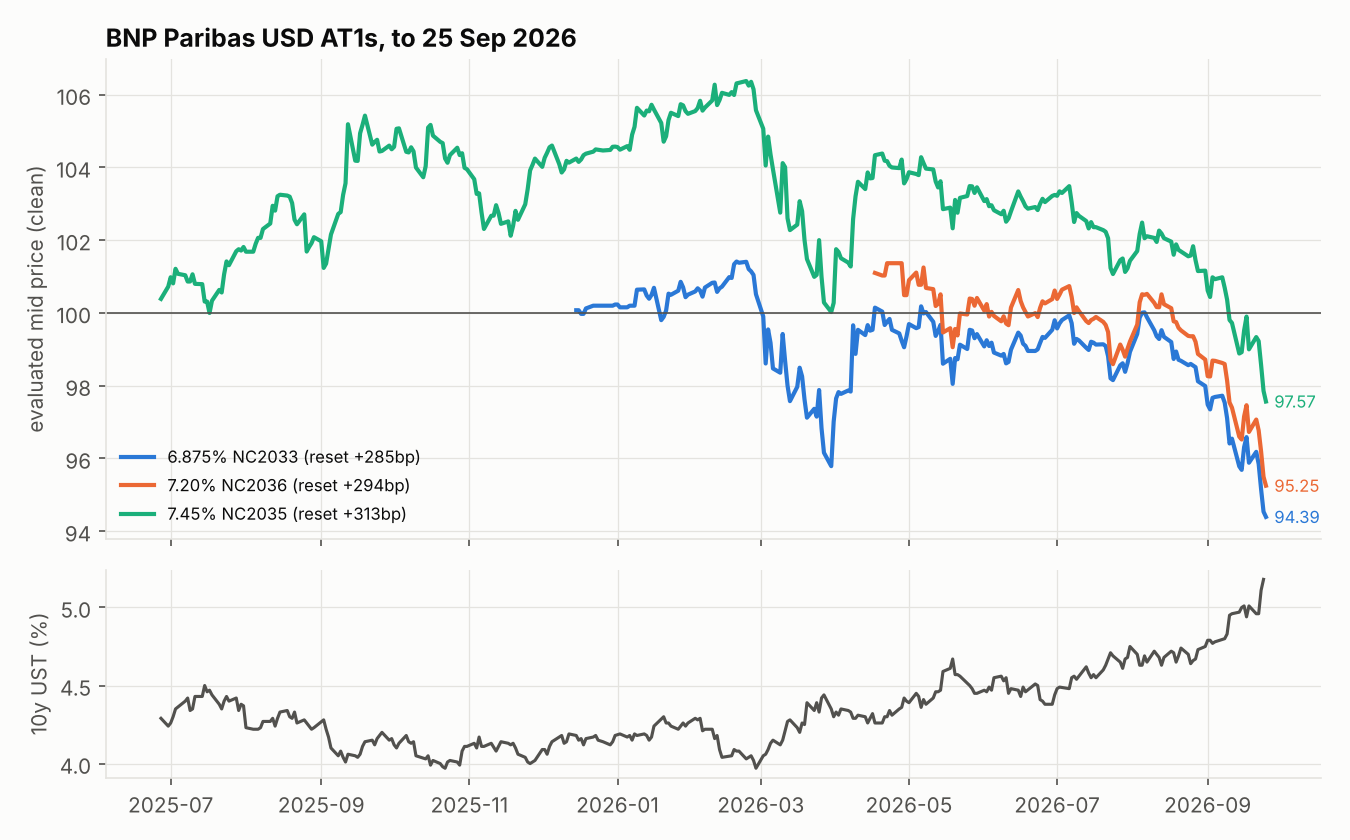
\includegraphics[width=0.92\textwidth]{bnp_at1_prices.png}
\caption{BNP Paribas USD AT1s: Capital IQ evaluated mid prices.}
\label{fig:prices}
\end{figure}
%======================================================================
\section{The model}\label{sec:model}
%======================================================================

\subsection{Probability space and measures}

Fix a filtered probability space $(\Omega,\F,(\F_t)_{t\ge0},\Q)$ satisfying the usual
conditions, supporting two standard Brownian motions $W$ and $B$ with
$\dd\langle W,B\rangle_t=\rho\dd t$, a Poisson process $N$ with intensity $\lambda_J$,
an i.i.d.\ sequence of jump sizes $(J_n)_{n\ge1}$, and two unit exponential random
variables $E_{\mathrm{res}}$ and $E_{\mathrm{spec}}$. The Brownian motions, the
compound Poisson process and the exponentials are mutually independent, except for the
correlation between $W$ and $B$. Denote by $\G=(\G_t)$ the filtration generated by
$(W,B,N,(J_n))$, the information in the state paths, and by
$\G_\infty=\bigvee_t\G_t$ its terminal $\sigma$-algebra.

All prices are expectations under $\Q$, a pricing measure. The CET1 ratio is not a
traded asset and its dynamics are estimated from quarterly history, that is under the
physical measure $\Prob$.

\begin{assumption}[Capital dynamics under the pricing measure]\label{ass:measure}
The dynamics of the CET1 ratio are the same under $\Q$ and under $\Prob$. All risk
premia not captured by the mechanical features of the contract are absorbed by the
write-down hazard $\lambda$, which is therefore a risk-neutral intensity and not a
probability of default.
\end{assumption}

Assumption~\ref{ass:measure} is the standard compromise of reduced-form models
calibrated to an untraded state variable. Its consequence is that $\lambda$ should be
read as a price, not as a forecast: a hazard of $2.2\%$ a year is the compensation the
market requires for the write-down risk and its premium, not a $2.2\%$ annual
probability of write-down.

\subsection{The CET1 ratio}

Let $C_t$ be the CET1 ratio in percentage points. It follows the mean-reverting
jump-diffusion
\begin{equation}\label{eq:cet1}
  \dd C_t = \kappa(\theta-C_t)\dd t + \sigma\dd W_t - \dd L_t,
  \qquad L_t=\sum_{n=1}^{N_t}J_n,
\end{equation}
with $\kappa>0$, $\sigma>0$, and lognormal jump sizes with mean $m_J$,
\begin{equation}\label{eq:jumps}
  J_n = m_J\exp\!\bigl(\sigma_J Z_n-\tfrac12\sigma_J^2\bigr),\qquad Z_n\sim N(0,1),
  \qquad \E[J_n]=m_J,\quad \E[J_n^2]=m_J^2e^{\sigma_J^2}.
\end{equation}
The drift represents capital management: retained earnings, distribution policy and
the management of risk-weighted assets pull the ratio back to the target $\theta$, the
CET1 objective the bank communicates to investors. Jumps are one-sided because losses
(a fine, a trading loss, an impairment, a regulatory change in risk weights) arrive
suddenly, while capital is rebuilt gradually.

\begin{proposition}[Solution and moments]\label{prop:cet1}
Equation~\eqref{eq:cet1} has the unique strong solution
\begin{equation}\label{eq:cet1sol}
  C_t = \theta + (C_0-\theta)e^{-\kappa t}
  + \sigma\int_0^t e^{-\kappa(t-u)}\dd W_u
  - \int_0^t e^{-\kappa(t-u)}\dd L_u ,
\end{equation}
with mean and variance
\begin{align}
  \E[C_t] &= \theta + (C_0-\theta)e^{-\kappa t} - \frac{\lambda_J m_J}{\kappa}\bigl(1-e^{-\kappa t}\bigr),
  \label{eq:cet1mean}\\
  \operatorname{Var}[C_t] &= \frac{\sigma^2+\lambda_J m_J^2e^{\sigma_J^2}}{2\kappa}\bigl(1-e^{-2\kappa t}\bigr).
  \label{eq:cet1var}
\end{align}
As $t\to\infty$, $C_t$ converges in distribution to a stationary law with mean
$\theta-\lambda_Jm_J/\kappa$ and variance $(\sigma^2+\lambda_Jm_J^2e^{\sigma_J^2})/(2\kappa)$.
\end{proposition}

\begin{proof}
The coefficients are affine with Lipschitz drift and constant diffusion, so a unique
strong solution exists. Apply It\^o's formula for semimartingales to
$e^{\kappa t}C_t$: $\dd(e^{\kappa t}C_t)=e^{\kappa t}(\kappa\theta\dd t+\sigma\dd W_t-\dd L_t)$,
and integrate to obtain \eqref{eq:cet1sol}. For the mean, the stochastic integral against
$W$ has zero expectation, and
$\E\int_0^te^{-\kappa(t-u)}\dd L_u=\lambda_Jm_J\int_0^te^{-\kappa(t-u)}\dd u$ by the
compensator of the compound Poisson process. For the variance, the Brownian and jump
integrals are independent; It\^o's isometry gives
$\sigma^2\int_0^te^{-2\kappa(t-u)}\dd u$ for the first, and the isometry for compensated
compound Poisson integrals gives $\lambda_J\E[J^2]\int_0^te^{-2\kappa(t-u)}\dd u$ for the
second. Evaluating the integrals gives \eqref{eq:cet1mean}--\eqref{eq:cet1var}. The
characteristic function of \eqref{eq:cet1sol} converges as $t\to\infty$, which gives
the stationary law.
\end{proof}

\begin{remark}[Target and long-run mean]\label{rem:target}
The long-run mean is not $\theta$ but $\theta-\lambda_Jm_J/\kappa$: jumps pull the ratio
down on average, and mean reversion offsets them only partially. With the base-case
parameters ($\theta=13\%$, $\kappa=0.35$, $\lambda_J=0.12$, $m_J=2.2$pp) the stationary
mean is $12.25\%$, and the stationary standard deviation is $1.17$pp, of which the
diffusion alone contributes $\sigma/\sqrt{2\kappa}=0.56$pp. Interpreting $\theta$ as
the bank's target is therefore accurate in the absence of shocks; in the presence of
shocks, the model's capital hovers about $0.75$pp below target on average. A calibration
that wanted the long-run mean, rather than the shock-free target, to equal $13\%$ would set
$\theta=13.75\%$; we keep $\theta$ at the communicated target and report the implication.
\end{remark}

The mechanical trigger time is the first passage
\begin{equation}
  \tau_m = \inf\{t\ge0:\ C_t\le \ctrig\},\qquad \ctrig=5.125\%.
\end{equation}

\subsection{The refinancing spread}

Let $S_t$ be the market component of the issuer's new-issue AT1 spread, in decimal.
It follows the Ornstein--Uhlenbeck process
\begin{equation}\label{eq:spread}
  \dd S_t = a(\bar s-S_t)\dd t + \eta\dd B_t,
\end{equation}
correlated with the diffusive capital shocks through $\rho<0$: when capital falls,
spreads tend to widen. The issuer's effective spread adds a capital premium once the
CET1 ratio enters the buffer,
\begin{equation}\label{eq:seff}
  s_t = S_t + \beta\bigl(\cmda(t)-C_t\bigr)^+ ,
\end{equation}
where $\cmda(t)$ is the MDA threshold defined in \eqref{eq:mdathreshold} below and $\beta$
is the extra spread per point of CET1 inside the buffer. The effective spread is the rate
at which the bank could issue a new AT1 at time $t$.

\begin{proposition}[Spread distribution]\label{prop:spread}
The solution of \eqref{eq:spread} is Gaussian,
\begin{equation}
  S_t = \bar s + (S_0-\bar s)e^{-at} + \eta\int_0^te^{-a(t-u)}\dd B_u
  \ \sim\ N\!\Bigl(\bar s + (S_0-\bar s)e^{-at},\ \frac{\eta^2}{2a}\bigl(1-e^{-2at}\bigr)\Bigr),
\end{equation}
and its covariance with the diffusive part of capital,
$C^W_t=\sigma\int_0^te^{-\kappa(t-u)}\dd W_u$, is
\begin{equation}\label{eq:covsc}
  \operatorname{Cov}\bigl(S_t,C^W_t\bigr) = \frac{\rho\sigma\eta}{a+\kappa}\Bigl(1-e^{-(a+\kappa)t}\Bigr).
\end{equation}
In the stationary regime $\Q(S_t<0)=\Phi\bigl(-\bar s\sqrt{2a}/\eta\bigr)$.
\end{proposition}

\begin{proof}
The solution follows as in Proposition~\ref{prop:cet1}. The covariance follows from
It\^o's isometry for two Wiener integrals:
$\E[\int_0^tf\dd B\int_0^tg\dd W]=\rho\int_0^tf(u)g(u)\dd u$ with
$f(u)=\eta e^{-a(t-u)}$ and $g(u)=\sigma e^{-\kappa(t-u)}$.
\end{proof}

With the base-case parameters ($a=0.5$, $\bar s=275$bp, $\eta=100$bp) the stationary
standard deviation of $S$ is $100$bp and the stationary probability of a negative spread
is $0.3\%$. Because the hazard and the call rule use the spread, negative values are
handled explicitly: the hazard is floored at zero (equation~\eqref{eq:hazard}), and a
negative refinancing spread simply triggers a call. A square-root or log-normal spread
would avoid negative values at the cost of the exact Gaussian transition; at a
probability of $0.3\%$ the difference is immaterial.

\subsection{The regulatory threshold}

Let $b$ be the MDA floor (Pillar~1 plus the CET1 part of Pillar~2R) and $w(t)$ the
combined buffer at time $t$. The MDA threshold is
\begin{equation}\label{eq:mdathreshold}
  \cmda(t) = b + w(t),\qquad w(t)=w_0+\sum_k \Delta w_k\,\1\{t\ge t_k\},
\end{equation}
where the steps $(t_k,\Delta w_k)$ are scheduled buffer changes. For BNP, $b=5.64\%$,
$w_0=4.79\%$ (so that $\cmda(0)$ equals the published requirement of $10.43\%$), and the
O-SII step-ups give $\Delta w=0.25$pp on 1 January 2027 and on 1 January 2028.

\subsection{Contract features as functionals of the state}

\paragraph{MDA coupon restriction.} With $q_t=(C_t-b)/w(t)$ the position of the ratio
inside the buffer, the fraction of the scheduled coupon that can be paid is
\begin{equation}\label{eq:mda}
  \phi(C_t,t)=
  \begin{cases}
    1 & C_t\ge \cmda(t),\\
    0.6 & q_t\in[0.75,1),\\
    0.4 & q_t\in[0.50,0.75),\\
    0.2 & q_t\in[0.25,0.50),\\
    0 & q_t<0.25.
  \end{cases}
\end{equation}
This applies the MDA quartile factors to the coupon itself. It is a stylised and
conservative version of the rule, which caps all distributions together
(Section~\ref{sec:institutions}); the resulting MDA component of the spread is an upper
bound.

\paragraph{Call and extension.} Let $T_1<T_2<\dots$ be the reset dates and $m$ the reset
margin. The issuer calls at
\begin{equation}\label{eq:call}
  \tau_c = \min\bigl\{T_k:\ m> s_{T_k}-\delta,\ \ C_{T_k}\ge\cmda(T_k),\ \ T_k<\tau_m\bigr\}
  \qquad(\min\emptyset=+\infty),
\end{equation}
that is, at the first reset date at which keeping the bond costs more than refinancing
it, less a reputational tolerance $\delta\ge0$, provided that the regulator would approve
the call (CET1 above the threshold) and the bond is still alive. In the base case
$\delta=0$. Since each condition is $\G_{T_k}$-measurable, $\tau_c$ is a $\G$-stopping
time taking values in $\{T_k\}\cup\{+\infty\}$. If $\eta>0$ the call is random even for a
healthy bank, and the bond with the lowest margin is the first to be extended when
spreads widen.

\paragraph{Conversion.} At $\tau_m$ the bond converts into shares at the higher of the
market price and the floor price $P_{\mathrm{floor}}$. When the share trades below the
floor, as it will at the trigger, the investor receives
$F\cdot S^{\mathrm{eq}}_{\tau_m}/P_{\mathrm{floor}}$. We do not model the share price
jointly with capital; instead the share price at conversion is a fixed fraction $\xi$ of
today's price $S^{\mathrm{eq}}_0$ converted at today's exchange rate $X_0$, so the recovery
at conversion is
\begin{equation}\label{eq:conv}
  R_{\mathrm{conv}}=\min\!\left(1,\ \frac{\xi\,S^{\mathrm{eq}}_0X_0}{P_{\mathrm{floor}}}\right).
\end{equation}
With $\xi=0.2$, a share price of EUR~98.43 and $X_0=1.15$, $R_{\mathrm{conv}}$ is $37\%$
for the 6.875\% and the 7.45\% and $31\%$ for the 7.20\%, whose floor is higher.

\subsection{The write-down hazard}\label{sec:hazard}

The regulator may impose losses before the trigger. We model the PONV time as a
doubly-stochastic (Cox) time with intensity proportional to the effective spread,
\begin{equation}\label{eq:hazard}
  \lambda_t = \lambda\,\frac{s_t^+}{s_0},\qquad
  I_t=\int_0^t\frac{s_u^+}{s_0}\dd u ,
\end{equation}
so that $\lambda$ is today's hazard and $I_t$ is the integrated driver. The hazard rises
when spreads widen or capital falls inside the buffer. The recovery of the AT1 at PONV is
zero.

Linking the hazard to $s_t$ is what makes extension consistent. The issuer extends when
$s_t>m$; with a state-dependent hazard those are exactly the states in which the bond is
riskier, and the extended cash flows are discounted accordingly. With a constant hazard,
the extended coupon $y^{\mathrm{ref}}+m$ would be discounted at a rate that does not reflect
the state, and in states where $m$ exceeds the risk-adjusted discount spread, not calling
would add value for the investor. Section~\ref{sec:robust} shows the size of this effect.

\subsection{Two clocks: resolution and AT1-specific write-down}\label{sec:twoclocks}

To price the AT1 jointly with the bank's Tier~2, decompose the hazard level into
\begin{equation}\label{eq:split}
  \lambda=\lres+\lspec,\qquad \lres,\lspec\ge0,
\end{equation}
and define two write-down times with the same driver,
\begin{equation}\label{eq:clocks}
  \tau_{\mathrm{res}} = \inf\{t:\ \lres I_t\ge E_{\mathrm{res}}\},\qquad
  \tau_{\mathrm{spec}} = \inf\{t:\ \lspec I_t\ge E_{\mathrm{spec}}\}.
\end{equation}
The resolution time $\tau_{\mathrm{res}}$ imposes losses on AT1 and on Tier~2; the
AT1-specific time $\tau_{\mathrm{spec}}$ imposes losses on AT1 alone. The AT1 write-down
time is $\tau_P=\tau_{\mathrm{res}}\wedge\tau_{\mathrm{spec}}$.

\begin{proposition}[Joint survival]\label{prop:clocks}
Conditionally on $\G_\infty$,
\begin{align}
  \Q(\tau_P>t\mid\G_\infty) &= e^{-\lambda I_t},\label{eq:survat1}\\
  \Q(\tau_{\mathrm{res}}>t\mid\G_\infty) &= e^{-\lres I_t},\label{eq:survt2}\\
  \Q(\tau_{\mathrm{res}}\le t,\ \tau_{\mathrm{res}}\le\tau_{\mathrm{spec}}\mid\G_\infty)
  &= \frac{\lres}{\lambda}\bigl(1-e^{-\lambda I_t}\bigr).\label{eq:firstres}
\end{align}
In particular $\tau_P$ is a Cox time with intensity $\lambda s_t^+/s_0$, and the
probability that an AT1 write-down is a resolution event that also hits Tier~2 is
$\lres/\lambda$, independently of the path.
\end{proposition}

\begin{proof}
$I_t$ is $\G_\infty$-measurable, continuous and non-decreasing, and the exponentials are
independent of $\G_\infty$ and of each other. Hence
$\Q(\tau_{\mathrm{res}}>t\mid\G_\infty)=\Q(E_{\mathrm{res}}>\lres I_t\mid\G_\infty)=e^{-\lres I_t}$,
which is \eqref{eq:survt2}; the same holds for $\tau_{\mathrm{spec}}$ with $\lspec$, and by
conditional independence $\Q(\tau_P>t\mid\G_\infty)=e^{-\lres I_t}e^{-\lspec I_t}$,
which is \eqref{eq:survat1}. For \eqref{eq:firstres}, change time to
$u=I_t$: conditionally on $\G_\infty$, $\tau_{\mathrm{res}}$ and $\tau_{\mathrm{spec}}$
become independent exponential times in $u$ with rates $\lres$ and $\lspec$, and the
probability that the first of two independent exponentials occurs before $u$ and is the
one with rate $\lres$ is $\frac{\lres}{\lambda}(1-e^{-\lambda u})$.
\end{proof}

Proposition~\ref{prop:clocks} is the formal content of the Tier~2 anchor. The AT1 price
depends on $\lres$ and $\lspec$ only through their sum, so the AT1 alone cannot separate
them; the Tier~2 depends on $\lres$ alone and identifies it. The ratio $\lres/\lambda$ is
the share of AT1 write-down risk that the market prices in Tier~2 as well.

Two remarks on interpretation. First, $\lres$ is calibrated to the Tier~2 spread, which
also contains the risk and liquidity premia that investors require on Tier~2 itself.
``Priced in Tier~2'' is therefore the accurate label for $\lres$; ``bank resolution
risk'' is an approximation. Second, the construction assumes that resolution hits AT1
whenever it hits Tier~2, which is the creditor hierarchy, and allows AT1-only write-downs
of the Credit Suisse type through $\tau_{\mathrm{spec}}$. It rules out a Tier~2 loss
without an AT1 loss, which the hierarchy also rules out.

%======================================================================
\section{Valuation}\label{sec:valuation}
%======================================================================

\subsection{The pricing equation}

Let $r$ be the flat, continuously compounded risk-free rate used for discounting, $F$ the
face value, $f$ the coupon frequency and $t_1<t_2<\dots$ the coupon dates. The scheduled
coupon rate is $c(t_i)=c_0$ up to and including the first reset $T_1$ and
$c(t_i)=y^{\mathrm{ref}}+m$ after it, where $y^{\mathrm{ref}}$ is the five-year reference
rate. A coupon is paid if the bond has not been converted, called or written down, scaled
by the MDA fraction. The principal is repaid at the call, converted at the trigger, or
lost at PONV. The dirty price at time 0 is
\begin{equation}\label{eq:price}
\begin{split}
  V_0=\E\Biggl[\,&\sum_{t_i\le H}\1_{\{t_i<\tau_m,\ t_i\le\tau_c,\ t_i<\tau_P\}}
  \,\phi(C_{t_i},t_i)\,\frac{c(t_i)F}{f}\,e^{-rt_i}
  + \1_{\{\tau_c<\tau_m\wedge\tau_P,\ \tau_c\le H\}}\,F\,e^{-r\tau_c}\\
  &+ \1_{\{\tau_m<\tau_c\wedge\tau_P,\ \tau_m\le H\}}\,R_{\mathrm{conv}}F\,e^{-r\tau_m}
  + \1_{\{\tau_c\wedge\tau_m\wedge\tau_P>H\}}\,T_H\,e^{-rH}\Biggr],
\end{split}
\end{equation}
where $H$ is the simulation horizon and $T_H$ the value at $H$ of a bond still alive,
\begin{equation}\label{eq:tail}
  T_H = \frac{(y^{\mathrm{ref}}+m)F}{r+\lambda\, s_H^+/s_0}.
\end{equation}
The tail is the value of a perpetuity paying the reset coupon continuously, discounted
at the risk-free rate plus the hazard frozen at its level at $H$. With $H=40$ years and
$r\approx5\%$, the tail is discounted by $e^{-rH}\approx0.13$ and weighted by the
probability of survival without call to year 40, which is below $3\%$ in the base case
(Table~\ref{tab:callext}); its contribution to the price is a few hundredths of a point.

\subsection{Conditional Monte Carlo}

The write-down time enters \eqref{eq:price} only through the indicators
$\1_{\{t<\tau_P\}}$. Every other quantity is a functional of the state paths.

\begin{theorem}[Conditional pricing formula]\label{thm:cmc}
Let $\mathrm{CF}_i$ be the coupon cash flows of \eqref{eq:price} with the indicator of
$\tau_P$ removed, and let $\mathrm{CF}_{\mathrm{end}}$ and $T_{\mathrm{end}}$ be the
redemption, conversion or tail payment and its date on each path. Then
\begin{equation}\label{eq:cmc}
  V_0(\lambda)=\E\Biggl[\,\sum_{i}\mathrm{CF}_i\,e^{-rt_i-\lambda I_{t_i}}
  + \mathrm{CF}_{\mathrm{end}}\,e^{-rT_{\mathrm{end}}-\lambda I_{T_{\mathrm{end}}}}\Biggr].
\end{equation}
\end{theorem}

\begin{proof}
All of $\mathrm{CF}_i$, $\mathrm{CF}_{\mathrm{end}}$, $T_{\mathrm{end}}$, $\tau_m$ and
$\tau_c$ are $\G_\infty$-measurable. By the tower property,
$\E[X\1_{\{t<\tau_P\}}]=\E[X\,\Q(\tau_P>t\mid\G_\infty)]=\E[Xe^{-\lambda I_t}]$ for any
$\G_\infty$-measurable integrable $X$, by \eqref{eq:survat1}. Apply this to each term of
\eqref{eq:price}. In the tail term the event $\{\tau_P>H\}$ contributes $e^{-\lambda I_H}$,
and the value of the perpetuity after $H$ is given by \eqref{eq:tail}.
\end{proof}

The estimator replaces the simulated indicator by its conditional expectation. Two
consequences follow.

\begin{proposition}[Variance reduction]\label{prop:var}
Let $X$ be the discounted payoff of \eqref{eq:price} on one path, with $\tau_P$
simulated, and $Y=\E[X\mid\G_\infty]$ the integrand of \eqref{eq:cmc}. Then
$\E[Y]=\E[X]$ and $\operatorname{Var}(Y)=\operatorname{Var}(X)-\E[\operatorname{Var}(X\mid\G_\infty)]\le\operatorname{Var}(X)$,
with equality only if $X$ is $\G_\infty$-measurable.
\end{proposition}

\begin{proof}
This is the law of total variance.
\end{proof}

\begin{proposition}[Shape of the price in the hazard]\label{prop:shape}
On any fixed set of paths, and in expectation, the map $\lambda\mapsto V_0(\lambda)$ on
$[0,\infty)$ is infinitely differentiable, strictly decreasing and strictly convex, with
\begin{equation}\label{eq:dv}
  V_0'(\lambda) = -\E\Bigl[\sum_i\mathrm{CF}_i\,I_{t_i}e^{-rt_i-\lambda I_{t_i}}
  + \mathrm{CF}_{\mathrm{end}}\,I_{T_{\mathrm{end}}}e^{-rT_{\mathrm{end}}-\lambda I_{T_{\mathrm{end}}}}\Bigr]
  + \text{(tail term)} <0,
\end{equation}
$V_0(\lambda)\to0$ as $\lambda\to\infty$. Consequently, for any market price
$P\in(0,V_0(0))$ the implied hazard $\lambda^\star$ solving $V_0(\lambda^\star)=P$ exists
and is unique, and any bracketing method on $[0,\bar\lambda]$ with
$V_0(\bar\lambda)<P$ converges to it.
\end{proposition}

\begin{proof}
Each summand has the form $a\,e^{-\lambda b}$ with $a\ge0$ and $b=I_t>0$ for $t>0$. The
driver starts at $s_0/s_0=1$ (when CET1 is above the threshold) and is continuous, so
$I_t>0$ for every $t>0$ on every path. Each summand is therefore smooth, decreasing and
convex in $\lambda$, strictly so when $a>0$. The tail summand is the product of
$(y^{\mathrm{ref}}+m)F/(r+\lambda d)$ and $e^{-\lambda I_H}$ with $d=s_H^+/s_0\ge0$; both
factors are positive, decreasing and convex, and for two such functions
$(gh)''=g''h+2g'h'+gh''\ge0$ since $g'h'\ge0$. Sums and averages preserve these
properties, and at least one coupon is positive with positive probability, which gives
strictness. Every summand vanishes as $\lambda\to\infty$; dominated convergence gives the
limit. Existence and uniqueness of the root follow from continuity and strict
monotonicity.
\end{proof}

In practice we solve $V_0(\lambda)=P^{\mathrm{clean}}+\mathrm{AI}$ with Brent's method
\citep{Brent1973} on $[0,1]$. Because the path-wise cash flows and the integrated
drivers are stored once, each evaluation of $V_0(\lambda)$ is a vectorised sum, and the
root costs a few milliseconds. Proposition~\ref{prop:shape} also gives the price
sensitivity to the hazard, which we use in Section~\ref{sec:calibration} to translate
hazard differences into price units: for the three AT1s $|V_0'|$ is $0.077$--$0.084$
points per basis point of hazard.

\subsection{Monte Carlo error of the implied hazard}

Let $\hat V_n(\lambda)$ be the sample mean of $n$ paths. By the delta method, the
standard error of the implied hazard is approximately
\begin{equation}\label{eq:sehazard}
  \operatorname{se}(\hat\lambda^\star)\approx\frac{\operatorname{se}\bigl(\hat V_n(\lambda^\star)\bigr)}{\bigl|V_0'(\lambda^\star)\bigr|}.
\end{equation}
With $n=20{,}000$ paths, the standard error of the dirty price is $0.05$--$0.06$ points
and that of the implied hazard is $0.67$bp for all three bonds
(Appendix~\ref{app:numerics}). Because the three bonds are priced on the same paths, their
Monte Carlo errors are strongly positively correlated, and the cross-bond dispersion of
the implied hazards is more precise than each hazard: across independent seeds and path
counts from $5{,}000$ to $40{,}000$, the dispersion stays within $2.0$--$3.2$bp. The time
step matters more than the number of paths: on a fortnightly grid the dispersion is
$4.6$bp (Appendix~\ref{app:numerics}).

\subsection{Tier~2 and senior bonds}\label{sec:t2}

A Tier~2 or senior non-preferred note with coupons $c_i$ to a call date $T$ treated as
certain, recovery $R$ at resolution and resolution hazard $\lres s_t^+/s_0$ pays its
coupons and principal if $\tau_{\mathrm{res}}>T$, and $RF$ at $\tau_{\mathrm{res}}$ if
$\tau_{\mathrm{res}}\le T$.

\begin{proposition}[Tier~2 price]\label{prop:t2}
With recovery paid at the resolution time,
\begin{equation}\label{eq:t2cont}
  B_0=\E\Biggl[\sum_{t_i\le T}c_iF\,e^{-rt_i-\lres I_{t_i}}+F\,e^{-rT-\lres I_T}
  + RF\int_0^Te^{-ru}\,\lres\frac{s_u^+}{s_0}\,e^{-\lres I_u}\dd u\Biggr].
\end{equation}
On a grid $0=u_0<u_1<\dots<u_N=T$ with recovery paid at the end of the step in which
resolution occurs, the recovery leg is exactly
\begin{equation}\label{eq:t2grid}
  RF\sum_{n=0}^{N-1}\Bigl(e^{-\lres I_{u_n}}-e^{-\lres I_{u_{n+1}}}\Bigr)e^{-ru_{n+1}} ,
\end{equation}
and the difference from \eqref{eq:t2cont} is bounded by $RF\bigl(1-e^{-r\Delta}\bigr)$.
\end{proposition}

\begin{proof}
The survival terms follow as in Theorem~\ref{thm:cmc} with \eqref{eq:survt2}. For the
recovery leg, conditionally on $\G_\infty$ the law of $\tau_{\mathrm{res}}$ has density
$\lres(s_u^+/s_0)e^{-\lres I_u}$, so
$\E[RFe^{-r\tau_{\mathrm{res}}}\1_{\{\tau_{\mathrm{res}}\le T\}}\mid\G_\infty]$ is the
integral in \eqref{eq:t2cont}. On the grid, the conditional probability of resolution in
$(u_n,u_{n+1}]$ is $e^{-\lres I_{u_n}}-e^{-\lres I_{u_{n+1}}}$, which gives
\eqref{eq:t2grid}. Paying at $u_{n+1}$ instead of at the resolution time within the step
changes the discount factor by at most a factor $e^{-r\Delta}$, and the total probability
of resolution is at most one.
\end{proof}

With a monthly grid and $r\approx5\%$ the bound is $0.4\%$ of the recovered amount, that
is about $0.01$ points for a recovery of $20\%$ and a resolution probability of about
$13\%$ to the call. The price \eqref{eq:t2grid} is again smooth and strictly
decreasing in $\lres$ for $R<1$, and the implied $\lres$ is unique. Crucially, the Tier~2
is priced on the \emph{same} paths and the same driver $I_t$ as the AT1s, so that $\lres$
and $\lambda$ are directly comparable.

\subsection{A term structure for the resolution hazard}\label{sec:piecewise}

A single level $\lres$ is calibrated to one Tier~2 bond. With two bonds of different
maturities we can bootstrap a piecewise-constant level,
$\lres(t)=\lambda_1\1\{t\le T^\ast\}+\lambda_2\1\{t>T^\ast\}$, where $T^\ast$ is the call of
the shorter bond. The integrated hazard becomes
$\int_0^t\lres(u)\frac{s_u^+}{s_0}\dd u=\lambda_1I_{t\wedge T^\ast}+\lambda_2\bigl(I_t-I_{T^\ast}\bigr)^+$.

\begin{lemma}\label{lem:piecewise}
Because $I$ is non-decreasing, $I_{t\wedge T^\ast}=\min(I_t,I_{T^\ast})$ and
$(I_t-I_{T^\ast})^+=\max(I_t-I_{T^\ast},0)$. Hence every price under the piecewise hazard
is computed from the stored values $I_{t_i}$ together with the single path-wise value
$I_{T^\ast}$.
\end{lemma}

The bootstrap is sequential: $\lambda_1$ is implied from the shorter bond, whose cash
flows end at $T^\ast$; $\lambda_2$ is then implied from the longer bond with $\lambda_1$
fixed; finally the AT1-specific level is implied from each AT1 with the piecewise
resolution hazard in place. Each step is a one-dimensional root with the monotonicity of
Proposition~\ref{prop:shape}.

\subsection{Discretisation}

The state is simulated on a monthly grid ($\Delta=1/12$) over $H=40$ years with
$20{,}000$ paths. The spread uses its exact Gaussian transition,
\begin{equation}
  S_{n+1}=\bar s+(S_n-\bar s)e^{-a\Delta}+\eta\sqrt{\frac{1-e^{-2a\Delta}}{2a}}
  \Bigl(\rho Z^C_n+\sqrt{1-\rho^2}\,Z^\perp_n\Bigr),
\end{equation}
where $Z^C_n$ is the normal of the CET1 step and $Z^\perp_n$ an independent normal. The
CET1 ratio uses an Euler step for the diffusion with a Bernoulli jump of probability
$1-e^{-\lambda_J\Delta}$ and lognormal size. The integrated driver uses the left-point rule,
$I_{n+1}=I_n+\Delta\,s^+_n/s_0$.

Three discretisation effects deserve comment. First, the Euler scheme for a linear SDE has
weak order one; with $\kappa\Delta\approx0.03$ the bias in the transition mean is of order
$(\kappa\Delta)^2/2\approx5\times10^{-4}$ in relative terms. Second, the trigger is
monitored only at grid dates, which underestimates the probability of crossing between
dates. \citet{BroadieGlassermanKou1997} show that, for a Brownian motion with volatility
$\sigma$, discrete monitoring is approximately equivalent to shifting the barrier away by
$0.5826\,\sigma\sqrt{\Delta}$; here the shift is $0.08$pp of CET1 against a distance of
$7.8$pp to the trigger, and the conversion component of the spread is only $4$bp, so the
effect is negligible. Third, events on the grid are read at grid dates, while coupons are
discounted at their exact dates. Halving the step to fortnightly changes the implied
hazards by at most $1.6$bp, but not by the same amount for every bond, so the cross-bond
dispersion rises from $2.6$ to $4.6$bp (Appendix~\ref{app:numerics}).

\subsection{Common random numbers}

All primitive random numbers are drawn once and reused across bonds, scenarios, bumps
and feature switches. A difference between two prices computed on the same paths
(a Greek, a stress P\&L, a component of the spread decomposition, the dispersion of the
implied hazards across bonds) therefore carries no Monte Carlo noise of its own beyond
the second-order effect of the change on the path-wise payoffs. This is what makes the
attribution of Section~\ref{sec:attribution} exact on a given set of paths.
%======================================================================
\section{Attributing the spread}\label{sec:attribution}
%======================================================================

The market quotes AT1 bonds by their yield to the first call over the matching
Treasury. We want to say how much of that spread pays for each risk. This section
defines the attribution and discusses its dependence on the order in which risks are
switched on.

\subsection{Features, prices and yields}

Index the risk features of the bond by the set
\[
  \mathcal N=\{\mathrm R,\mathrm S,\mathrm M,\mathrm C,\mathrm E\},
\]
standing for resolution hazard ($\lres$), AT1-specific hazard ($\lspec$), MDA coupon
restriction, conversion at the trigger, and extension (the economic call rule
\eqref{eq:call} instead of a certain call at $T_1$). For any subset $K\subseteq\mathcal N$
let $V(K)$ be the dirty price with exactly the features in $K$ switched on, computed on
the fixed set of paths:
\begin{itemize}
  \item hazard $(\lres\1_{\mathrm R\in K}+\lspec\1_{\mathrm S\in K})\,s^+_t/s_0$;
  \item coupons scaled by $\phi$ if $\mathrm M\in K$, paid in full otherwise;
  \item conversion at $\tau_m$ if $\mathrm C\in K$, no trigger otherwise;
  \item call by \eqref{eq:call} if $\mathrm E\in K$, certain call at $T_1$ otherwise.
\end{itemize}
$V(\emptyset)$ is the price of a risk-free bullet to $T_1$, and $V(\mathcal N)$ is the
model price, equal to the market price by calibration.

Let $y(V)$ be the semi-annual yield to the first call implied by a dirty price $V$,
treating the bond as a bullet to $T_1$, and define the spread of a subset as
$v(K)=y(V(K))-y(V(\emptyset))$. Because $V(\emptyset)$ is discounted at the risk-free
rate, $y(V(\emptyset))$ is the Treasury yield and $v(\mathcal N)$ is the market
yield-to-call spread. The map $V\mapsto y(V)$ is strictly decreasing, so $v$ is
increasing in risk.

\subsection{Sequential attribution and its order dependence}

Given an order $\pi=(\pi_1,\dots,\pi_5)$ of the features, the sequential attribution is
\begin{equation}\label{eq:sequential}
  \varphi^\pi_{\pi_k}=v(\{\pi_1,\dots,\pi_k\})-v(\{\pi_1,\dots,\pi_{k-1}\}),
\end{equation}
which telescopes to $\sum_k\varphi^\pi_{\pi_k}=v(\mathcal N)$: the components add up
exactly to the market spread. The attribution depends on $\pi$ whenever the features
interact, that is whenever $v$ is not additive. Interactions are pervasive here. The MDA
cuts coupons that would otherwise be paid only if the bond survives, so its cost depends on
the hazard; the value of the call option depends on the discount rate of the extended
cash flows, so its cost depends on the hazard and on the MDA; and the yield transformation
is non-linear.

The base attribution of the short note uses the order $(\mathrm R,\mathrm S,\mathrm M,\mathrm C,\mathrm E)$:
the hazard first, so that every contract feature is valued with risky discounting, and
extension last, so that the call is valued with every other feature in place.

\subsection{Shapley values}

The Shapley value \citep{Shapley1953} averages the sequential attribution over all
$|\mathcal N|!=120$ orders:
\begin{equation}\label{eq:shapley}
  \varphi^{\mathrm{Sh}}_j=\sum_{K\subseteq\mathcal N\setminus\{j\}}
  \frac{|K|!\,(|\mathcal N|-|K|-1)!}{|\mathcal N|!}\bigl(v(K\cup\{j\})-v(K)\bigr).
\end{equation}
It is the unique attribution satisfying efficiency ($\sum_j\varphi_j=v(\mathcal N)$),
symmetry (interchangeable features receive the same value), the null-player property
and additivity. It needs the $2^5=32$ values $v(K)$, which on a fixed set of paths require
only eight cash-flow profiles per bond (one for each combination of M, C and E): the two
hazard features enter through the discount exponent and are evaluated analytically.

The full Shapley value treats all orders as equally meaningful. For AT1 bonds they are
not. Orders in which extension is switched on before any hazard value the issuer's option
on a risk-free bond. When a risk-free bond pays its reset margin $m$ over Treasuries, not
calling it is a gift to the investor, so these orders assign extension a large negative
value; this is precisely the inconsistency that the state-dependent hazard of
Section~\ref{sec:hazard} is designed to avoid. We therefore also compute a Shapley value
within blocks.

\begin{definition}[Nested Shapley value]
Partition the features into the hazard block $\mathcal H=\{\mathrm R,\mathrm S\}$ and the
contract block $\mathcal K=\{\mathrm M,\mathrm C,\mathrm E\}$. The nested value is the
Shapley value of the game $v$ restricted to $\mathcal H$ for $j\in\mathcal H$, and the
Shapley value of the game $K\mapsto v(\mathcal H\cup K)-v(\mathcal H)$ on $\mathcal K$ for
$j\in\mathcal K$.
\end{definition}

The nested value is symmetric within each block and enters the hazard block first. It is
related to the value for games with a priori unions of \citet{Owen1977}, which would also
average over the order of the two blocks; we fix the order of the blocks for the economic
reason just given. By construction it is efficient: the hazard block receives
$v(\mathcal H)$ and the contract block $v(\mathcal N)-v(\mathcal H)$.

\begin{proposition}[Split of the hazard block]\label{prop:hazardsplit}
Within the hazard block, the nested value is
\[
  \varphi_{\mathrm R}=\tfrac12\bigl[v(\{\mathrm R\})+v(\mathcal H)-v(\{\mathrm S\})\bigr],\qquad
  \varphi_{\mathrm S}=\tfrac12\bigl[v(\{\mathrm S\})+v(\mathcal H)-v(\{\mathrm R\})\bigr].
\]
If the spread were linear in the hazard level on the relevant range,
$v(\{\mathrm R\})+v(\{\mathrm S\})=v(\mathcal H)$ and the nested value would coincide with
the sequential attribution in either order, giving
$\varphi_{\mathrm R}/(\varphi_{\mathrm R}+\varphi_{\mathrm S})=\lres/\lambda$.
\end{proposition}

\begin{proof}
The first statement is \eqref{eq:shapley} for two players. Under linearity
$v(\{\mathrm R\})=\lres\,g$ and $v(\{\mathrm S\})=\lspec\,g$ for some slope $g$, and both
orders give the same increments.
\end{proof}

For BNP the yield-to-call spread is very close to linear in the hazard on the relevant
range, so the split of the hazard block is effectively order-free: the nested value and
the base order agree to within $0.2$bp (Section~\ref{sec:robust}). The order matters for the
contract block, and there the attribution should be reported as a range.

%======================================================================
\section{Data and calibration}\label{sec:calibration}
%======================================================================

\subsection{Data}

\paragraph{Bond prices.} Daily Capital IQ evaluated bid, mid and ask prices for the three
AT1s, the two Tier~2 notes and the SNP note, from each bond's issue date (the earliest
being 27 June 2025) to 25 September 2026. Grey-market quotes before the issue date are
discarded, as are weekend repetitions of Friday's evaluation. The analysis uses weekly
(Friday) observations, 66 dates. Accrued interest is computed on a 30/360 basis on the
trade date and matches Capital IQ's ``T0 accrued interest'' to three decimals. Evaluated
prices are composites of dealer quotes rather than transactions; their bid--offer on the
valuation date is $0.15$--$0.29$ points for the AT1s and $0.07$--$0.17$ for the Tier~2 and
SNP notes, all of which carry Capital IQ's highest liquidity score.

\paragraph{Treasury curve.} FRED constant-maturity Treasury yields at five, seven and ten
years (DGS5, DGS7, DGS10). The five-year CMT is the reset reference of the AT1s; each bond is
discounted at the yield interpolated linearly at its time to first call, flat outside the
five-to-ten-year range.

\paragraph{Capital.} Quarterly CET1 ratios from Capital IQ, 2014Q1 to 2026Q2. Earlier data
follow Basel~II/2.5 definitions and are not comparable. A print is used only from 35 days
after the quarter end, approximating BNP's publication lag. The CET1 requirement is the
year-end stack from Capital IQ up to 2024 and the quarterly figures published by BNP
thereafter ($10.51\%$ at September 2025, $10.43\%$ at June 2026).

\paragraph{Credit default swaps.} BNP Paribas senior CDS, EUR, MM14 documentation:
the five-year conventional spread daily since October 2023 and full curves on six
snapshot dates. The CDS is used only as a reference point, because it is quoted in a
different currency and is referenced to senior rather than subordinated debt.

\paragraph{Other.} BNP's share price (EUR) and the EBA 2025 stress test results, in which
BNP's fully loaded CET1 ratio falls by $4.21$pp in the adverse scenario.

\subsection{Capital dynamics}

\paragraph{Likelihood.} Ignoring jumps, the CET1 process is an Ornstein--Uhlenbeck process
whose transition over a step $\Delta_k$ is Gaussian:
\begin{equation}\label{eq:outrans}
  C_{k+1}\mid C_k\sim N\bigl(m_k,\ \sigma^2w_k\bigr),\qquad
  m_k=\theta+(C_k-\theta)e^{-\kappa\Delta_k},\qquad
  w_k=\frac{1-e^{-2\kappa\Delta_k}}{2\kappa}.
\end{equation}
The exact log-likelihood of $n$ transitions is
\begin{equation}\label{eq:loglik}
  \ell(\kappa,\sigma)=-\frac12\sum_{k}\Bigl[\log\bigl(2\pi\sigma^2w_k\bigr)
  +\frac{(C_{k+1}-m_k)^2}{\sigma^2w_k}\Bigr].
\end{equation}
For fixed $\kappa$ the maximiser in $\sigma$ is available in closed form,
\begin{equation}\label{eq:sigmahat}
  \hat\sigma^2(\kappa)=\frac1n\sum_k\frac{(C_{k+1}-m_k)^2}{w_k},
\end{equation}
which gives the profile likelihood
$\ell_p(\kappa)=-\frac n2\bigl[1+\log(2\pi\hat\sigma^2(\kappa))\bigr]-\frac12\sum_k\log w_k$,
maximised numerically in $\kappa$. The long-run level is fixed at $\theta=13\%$, BNP's
communicated target; with fifty observations of a slowly mean-reverting series, a free
$\theta$ would be poorly determined and would interact with $\kappa$. The 2023Q1 transition
(+1.2pp, the sale of Bank of the West) is a disposal, not a capital shock, and is excluded
from the sum.

\paragraph{Estimates.} The maximum likelihood estimates are $\hat\kappa=0.165$ and
$\hat\sigma=0.44$pp$/\sqrt{\text{yr}}$, a half-life of a capital shock of $\ln2/\hat\kappa=4.2$
years. Figure~\ref{fig:cet1} shows the history, the requirement and the base-case outlook.

\begin{figure}[H]
\centering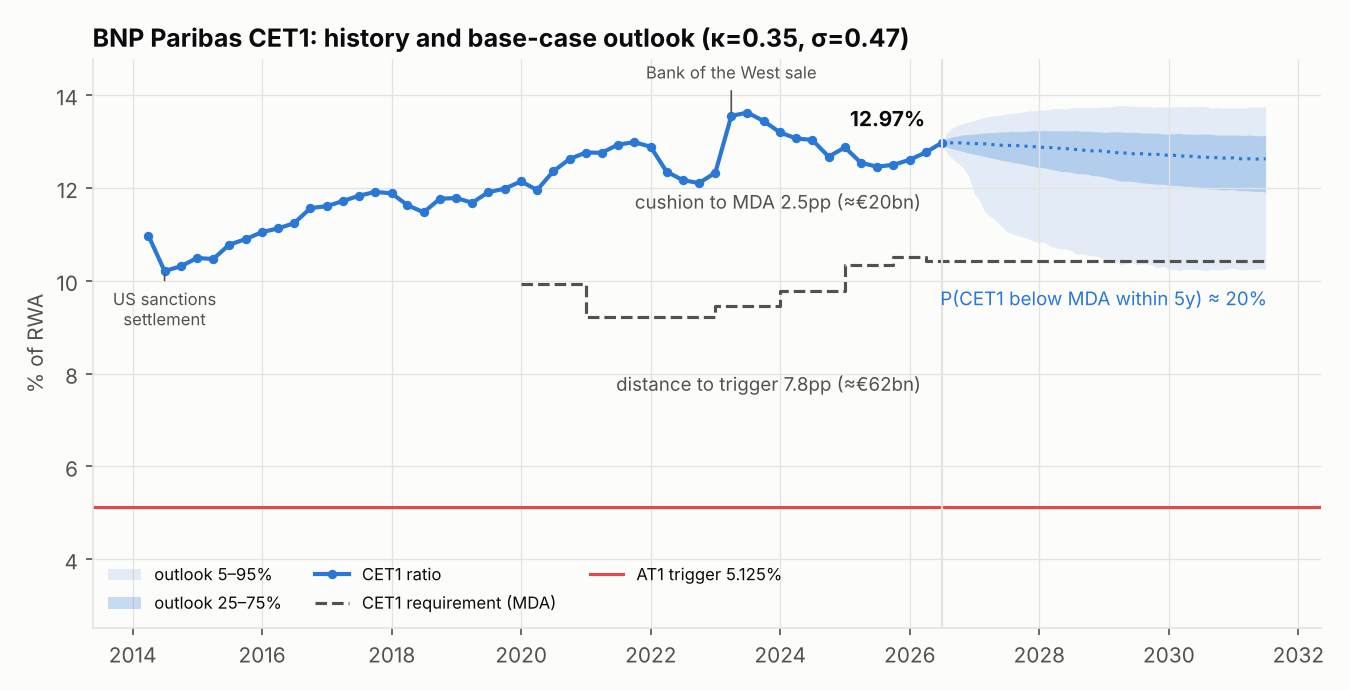
\includegraphics[width=0.85\textwidth]{bnp_cet1_history.png}
\caption{BNP Paribas CET1 ratio since 2014, CET1 requirement (MDA threshold), AT1 trigger
and the base-case five-year outlook (median, 50\% and 90\% bands of simulated CET1).}
\label{fig:cet1}
\end{figure}

\paragraph{Bootstrap.} To measure the precision of $\hat\kappa$ we simulate $1{,}000$
histories of the fitted process on the observed quarterly dates and re-estimate
$(\kappa,\sigma)$ on each. The $90\%$ intervals are $\kappa\in[0.063,\,0.476]$ and
$\sigma\in[0.37,\,0.52]$: the volatility is well identified, the speed of capital
rebuilding is not. The half-life of a capital shock lies between $1.5$ and $11$ years.
This is the familiar difficulty of estimating mean reversion from a short sample of a
persistent series, and it matters: Section~\ref{sec:uncert} shows that the capital stress
results scale by a factor of five across the interval.

\paragraph{Base case.} The base case uses $\kappa=0.35$ (half-life two years), inside the
bootstrap interval, with $\sigma=0.47$ re-estimated by \eqref{eq:sigmahat}. The
likelihood ratio statistic against the maximum likelihood estimate is $2\times1.5=3.0$,
below the $5\%$ critical value of $3.84$ for one restriction. Section~\ref{sec:uncert}
explains the choice: bond prices lean towards faster mean reversion, and BNP's explicit
capital management (a $13\%$ target with managed risk-weighted assets and distributions) is
consistent with it.

\paragraph{Jumps.} The jump parameters cannot be identified from fifty quarters with few
large shocks. We use $\lambda_J=0.12$ a year, $m_J=2.2$pp and $\sigma_J=0.5$. The $95$th
percentile of the jump size, $m_Je^{1.645\sigma_J-\sigma_J^2/2}=4.4$pp, matches the $4.2$pp
CET1 depletion of BNP in the EBA 2025 adverse scenario: the calibration says that a shock of
the size of the adverse scenario occurs as a single jump with probability
$0.12\times5\%=0.6\%$ a year, about once every 170 years; smaller jumps are more frequent and
can accumulate.

\subsection{Spread process and regulatory geometry}

The market component of the refinancing spread starts on each date at the average, across
the AT1s quoted that day, of the yield to first call minus the call-matched Treasury. It
mean-reverts at $a=0.5$ (half-life $1.4$ years) to the sample mean $\bar s=275$bp, with
volatility $\eta=100$bp and correlation $\rho=-0.3$ with capital shocks. The capital premium
is $\beta=1\%$ of spread per point of CET1 inside the buffer. Neither $\eta$ nor $\beta$
is identified by the data; Section~\ref{sec:results} reports the sensitivity of the
cross-section to $\eta$, and $\beta$ is discussed in Section~\ref{sec:discussion}. The MDA
geometry is as in \eqref{eq:mdathreshold}, the trigger is $5.125\%$, and the stressed share
price at conversion is $\xi=20\%$ of today's.

\subsection{Implied hazards and the cross-sectional test}

On each date and for each AT1 $j$ we solve $V^{(j)}_0(\lambda_j)=P_j^{\mathrm{clean}}+\mathrm{AI}_j$.
The three bonds share issuer, capital and trigger, so a correctly specified model should
give $\lambda_1=\lambda_2=\lambda_3$, and the dispersion
\[
  D=\max_j\lambda_j-\min_j\lambda_j
\]
is a specification test. It can also be used to ask which values of the unidentified
parameters ($\eta$, $\kappa$) the three prices are consistent with.

\paragraph{Power of the test.} The test has limited power with evaluated prices. By
Proposition~\ref{prop:shape}, a difference $\Delta\lambda$ in hazard corresponds to a price
difference of $|V_0'|\Delta\lambda$, with $|V_0'|=0.077$--$0.084$ points per basis point. The
bid--offer of $0.15$--$0.29$ points therefore corresponds to $1.9$--$3.5$bp of hazard. A
dispersion of a few basis points is within the precision of the data, and the test can
reject specifications that produce large dispersions but cannot rank specifications whose
dispersions differ by one or two basis points. Monte Carlo error is not the binding
constraint: the standard error of each implied hazard is $0.67$bp, and the dispersion,
computed on common random numbers, is more precise still.

\subsection{Tier~2 calibration and the identification of recovery}

On each date the Tier~2 and SNP notes are priced on the same simulated state as the AT1s,
with the spread process started at the same AT1 spread and the same CET1 print, and with
recoveries $R_{\mathrm{T2}}=20\%$ and $R_{\mathrm{SNP}}=40\%$, the Markit conventions for
subordinated and senior debt. Each bond gives an implied resolution hazard by
Proposition~\ref{prop:t2}; the Tier~2 2035NC34 is the anchor for $\lres$.

Recovery and hazard are not separately identified from a single bond: a higher recovery
requires a higher hazard to match the same price. With two bonds of the same tenor and
different seniority, Tier~2 and SNP, the restriction that both face the same resolution
hazard identifies one recovery given the other. We report the Tier~2 recovery $R^\star$
that equalises the two implied hazards given $R_{\mathrm{SNP}}=40\%$, and the sensitivity of
the AT1 split to $R_{\mathrm{T2}}$.

%======================================================================
\section{Results: BNP Paribas, 25 September 2026}\label{sec:results}
%======================================================================

All results are as of 25 September 2026. In the following month BNP's spreads widened
with French sovereign stress, the ten-year OAT yield rising above $5\%$: the senior CDS
five-year spread rose from 57 to 74bp and, in Capital IQ spreads to benchmark, the SNP from
98 to 122bp and the Tier~2 2035NC34 from 141 to 153bp by 27 October. The analysis does not
include that move.

\subsection{Capital}

CET1 was $12.97\%$ at June 2026 against a $10.43\%$ requirement: a cushion of $2.54$pp, about
EUR~20bn of losses at June 2026 risk-weighted assets of EUR~795bn. The trigger is $7.8$pp
below the ratio, about EUR~62bn of losses. Under the base-case dynamics, $20\%$ of the
simulated paths fall below the current MDA threshold at some point in the next five
years, while the trigger is almost never reached by diffusion alone. For these bonds
capital risk is first a coupon and call risk, and only then a conversion risk.

\subsection{The three bonds and the implied hazard}

Table~\ref{tab:implied} reports the implied hazards on the valuation date. Without
write-down risk the model would value the bonds at $114$--$118$, against market prices of
$94$--$98$: the mechanical features alone explain only a small part of the discount. The
implied hazards are $2.21\%$, $2.18\%$ and $2.19\%$ a year.

\begin{table}[H]
\centering
\begin{tabular}{lccc}
\toprule
 & 6.875\% NC33 & 7.20\% NC36 & 7.45\% NC35 \\
\midrule
Reset margin (bp) & 285 & 294 & 313 \\
Clean price & 94.39 & 95.25 & 97.57 \\
Bid--offer (points) & 0.26 & 0.29 & 0.15 \\
Yield-to-call spread (bp) & 279 & 274 & 269 \\
Model price with $\lambda=0$ & 114.2 & 116.9 & 117.6 \\
Implied hazard $\lambda$ (\%/yr) & 2.21 & 2.18 & 2.19 \\
Monte Carlo s.e.\ of $\lambda$ (bp) & 0.67 & 0.66 & 0.67 \\
$\Pr(\text{called at }T_1)$ & 49\% & 52\% & 58\% \\
$\Pr(\text{called at some reset})$ & 97\% & 98\% & 98\% \\
Lifetime $\Pr(\text{conversion})$ & 1.4\% & 1.6\% & 1.4\% \\
\bottomrule
\end{tabular}
\caption{Implied hazard and model outputs on 25 September 2026, base case ($\kappa=0.35$,
$\eta=100$bp, economic call rule).}
\label{tab:implied}
\end{table}

\paragraph{Cross-section.} Table~\ref{tab:eta} shows the dispersion of the three implied
hazards as a function of the spread volatility $\eta$. A deterministic refinancing spread
($\eta=0$) gives a dispersion of $8.2$bp; a stochastic one reduces it steadily, without an
interior minimum, so the cross-section does not identify $\eta$ and $100$bp is kept as an
assumption. In price terms the base-case dispersion of $2.6$bp is $0.20$--$0.22$ points, of
the size of the bid--offer: the bonds are consistent with one hazard within the precision
of the data.

\begin{table}[H]
\centering
\begin{tabular}{lccccccc}
\toprule
$\eta$ (bp) & 0 & 25 & 50 & 75 & 100 & 150 & 200\\
\midrule
Dispersion $D(\eta)$ (bp of hazard) & 8.2 & 5.8 & 4.1 & 3.0 & \textbf{2.6} & 2.0 & 1.4\\
In price points (6.875\%) & 0.63 & 0.45 & 0.32 & 0.23 & \textbf{0.20} & 0.15 & 0.11\\
\bottomrule
\end{tabular}
\caption{Cross-bond dispersion of the implied hazards on the valuation date, by
refinancing-spread volatility.}
\label{tab:eta}
\end{table}

Over the 66 weekly dates the mean dispersion is $5.9$bp with the stochastic spread and $9.3$bp
with the deterministic one. Priced at the day's common hazard, each bond's average pricing
error is within $\pm0.25$ points (range $-1.1$ to $+1.1$). Using Capital IQ benchmark yields
instead of the FRED curve, the last-date dispersion is $2.3$--$7.8$bp depending on the
benchmark assignment, so the choice of risk-free curve matters as much as the choice of
$\eta$. Figure~\ref{fig:implied} shows the implied hazards over time. The average hazard
ranged from $1.82\%$ (August 2026) to $2.69\%$ (late March 2026, when the bonds then
outstanding fell four to five points) and rose again into the September sell-off.

\begin{figure}[H]
\centering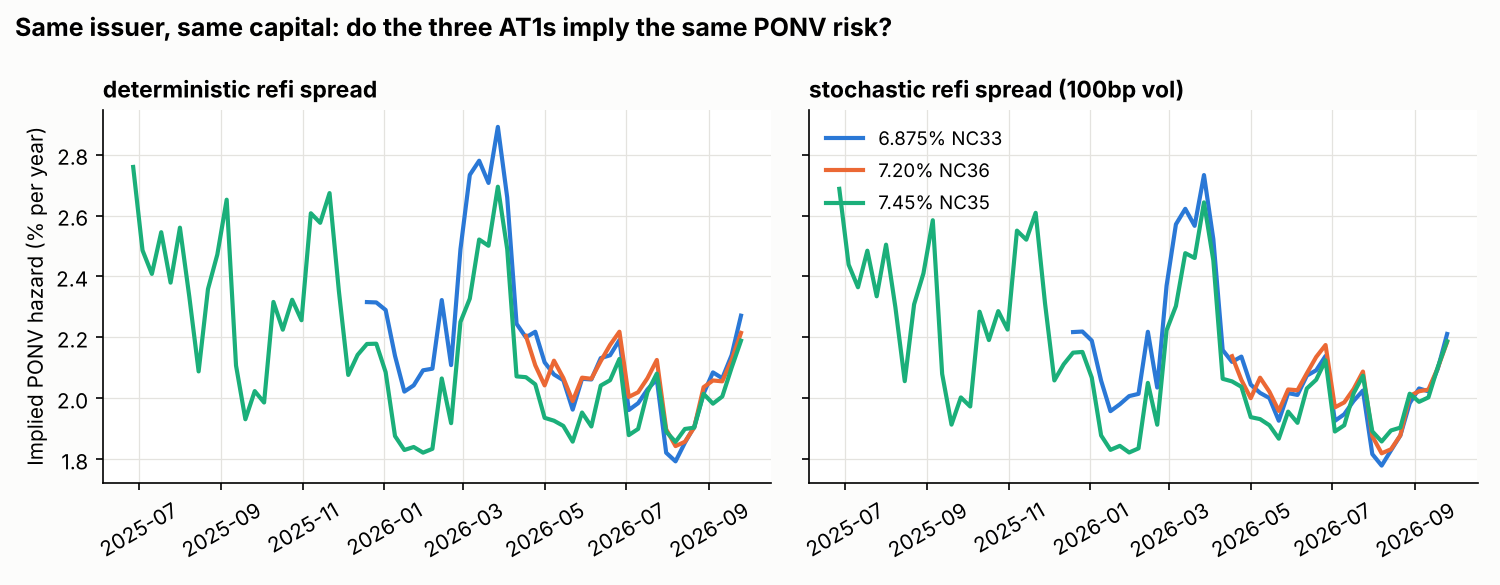
\includegraphics[width=\textwidth]{implied_ponv.png}
\caption{Implied hazard per bond, weekly, with a deterministic (left) and a stochastic
(right) refinancing spread.}
\label{fig:implied}
\end{figure}

\subsection{What BNP's Tier~2 prices}\label{sec:capstruct}

Table~\ref{tab:ladder} sets the AT1s against the rest of BNP's capital structure. Bond
hazards are implied on the same simulated state as the AT1s; CDS hazards use the credit
triangle $\lambda\approx s/(1-R)$.

\begin{table}[H]
\centering
\begin{tabular}{lcccc}
\toprule
 & Spread (bp) & Recovery & Hazard (\%/yr) & Share of AT1 hazard \\
\midrule
Senior CDS 5Y (EUR) & 57 & 40\% & 0.95 & 43\% \\
Senior CDS 7Y (EUR, 27 Sep) & 68 & 40\% & 1.13 & 52\% \\
Senior CDS 10Y (EUR, 27 Sep) & 81 & 40\% & 1.35 & 62\% \\
SNP 5.738\% 2035NC34 & 103 & 40\% & 1.63 & 74\% \\
T2 2.588\% 2035NC30 & 116 & 20\% & 1.40 & 64\% \\
\textbf{T2 5.906\% 2035NC34 (anchor)} & \textbf{144} & \textbf{20\%} & \textbf{1.72} & \textbf{78\%} \\
AT1 (average of three) & 274 & 0\% & 2.19 & 100\% \\
\bottomrule
\end{tabular}
\caption{BNP Paribas's capital structure on 25 September 2026. Bond spreads are yield to
call over the call-matched FRED Treasury.}
\label{tab:ladder}
\end{table}

The ladder is orderly: each step down the capital structure pays more. The two instruments
that share the resolution event, the Tier~2 and the SNP of the same tenor, imply nearly the
same hazard ($1.72\%$ and $1.63\%$) under the Markit recoveries. With the SNP at $40\%$, the
Tier~2 recovery that equalises the two is $R^\star=15.6\%$, close to the conventional $20\%$:
the prices of BNP's own bonds are consistent with the recovery conventions. The CDS sits
below the bonds, as one would expect of a EUR contract on senior debt compared with USD cash
bonds that carry funding and liquidity premia. The shorter Tier~2 implies a lower hazard than
the longer one, an upward-sloping term structure that Section~\ref{sec:robust} exploits.

With the Tier~2 2035NC34 as anchor,
\begin{equation}
  \lambda = 2.19\% = \underbrace{1.72\%}_{\lres:\ \text{priced in Tier~2}}
  + \underbrace{0.47\%}_{\lspec:\ \text{AT1-specific}} .
\end{equation}
By Proposition~\ref{prop:clocks}, $78\%$ of the AT1's write-down risk, in risk-neutral
terms, is compensation that BNP's Tier~2 also earns; the remaining $22\%$ is what the market
charges for being an AT1 rather than a Tier~2. Over the 66 weekly dates the Tier~2 share
ranges from $66\%$ to $80\%$, with a mean of $72\%$ (Figure~\ref{fig:capstruct}).

The two halves of this split are not equally robust. The Tier~2-priced hazard hardly depends
on the capital dynamics: re-solved on the paths of each value of $\kappa$ in its bootstrap
interval, $\lres$ ranges only from $1.61\%$ to $1.74\%$ a year. The AT1-specific hazard
absorbs almost all of the uncertainty about how fast the bank rebuilds capital, and is
$0.47\%$ only in the base case; Section~\ref{sec:uncert} shows that it lies between zero and
about $0.5\%$ over the range of $\kappa$ that history and the Tier~2 jointly admit.

\begin{table}[H]
\centering
\begin{tabular}{lccccc}
\toprule
Tier~2 recovery & 0\% & 10\% & 20\% & 30\% & 40\% \\
\midrule
$\lres$ (\%/yr) & 1.37 & 1.53 & 1.72 & 1.97 & 2.30 \\
$\lspec$ (\%/yr) & 0.82 & 0.67 & 0.47 & 0.23 & $-0.11$ \\
Tier~2 share of the AT1 hazard & 63\% & 70\% & 78\% & 90\% & 105\% \\
\bottomrule
\end{tabular}
\caption{Sensitivity of the split to the Tier~2 recovery.}
\label{tab:recovery}
\end{table}

The split depends on the Tier~2 recovery (Table~\ref{tab:recovery}). A recovery as high as
the senior one would leave a negative AT1-specific hazard, which is implausible; any
recovery up to $30\%$ attributes at least three-fifths of the AT1 hazard to what Tier~2 also
prices.

\begin{figure}[H]
\centering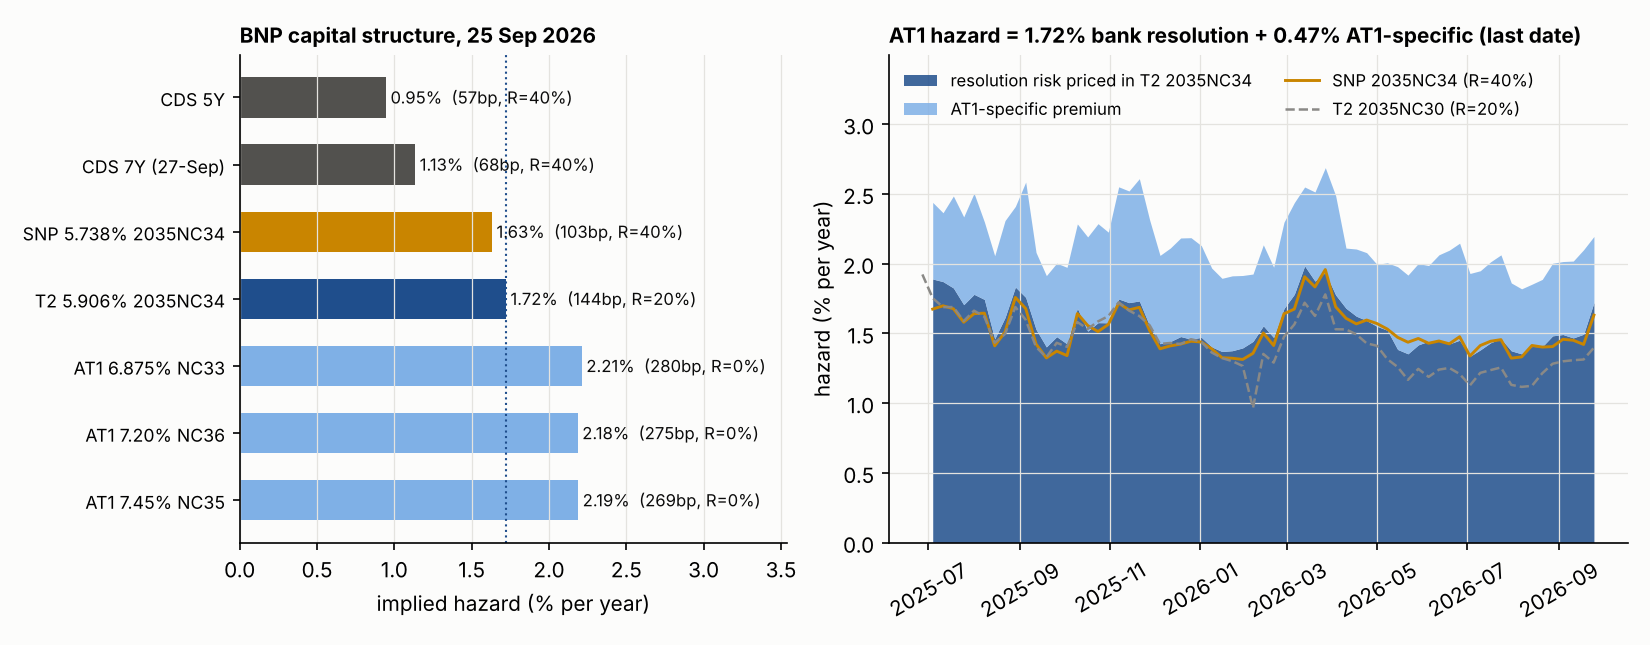
\includegraphics[width=\textwidth]{capital_structure.png}
\caption{Left: implied hazards down BNP's capital structure. Right: the AT1 hazard
(average of the three bonds), weekly, split into the part priced in the Tier~2 2035NC34
and the AT1-specific premium; the SNP and the shorter Tier~2 are shown for comparison.}
\label{fig:capstruct}
\end{figure}

\subsection{What the spread pays for}

Table~\ref{tab:decomp} and Figure~\ref{fig:decomp} give the base attribution of the
yield-to-call spread (order R, S, M, C, E).

\begin{table}[H]
\centering
\begin{tabular}{lccc}
\toprule
bp of yield-to-call spread & 6.875\% NC33 & 7.20\% NC36 & 7.45\% NC35 \\
\midrule
Priced in Tier~2 (resolution) & 181 & 181 & 180 \\
AT1-specific premium & 52 & 49 & 49 \\
MDA coupon cuts & 27 & 31 & 30 \\
Conversion at the trigger & 4 & 4 & 4 \\
Extension & 15 & 9 & 6 \\
\midrule
Total $=$ market & 279 & 274 & 269 \\
\bottomrule
\end{tabular}
\caption{Attribution of the yield-to-call spread, base order. Components are rounded to
sum to the total.}
\label{tab:decomp}
\end{table}

\begin{figure}[H]
\centering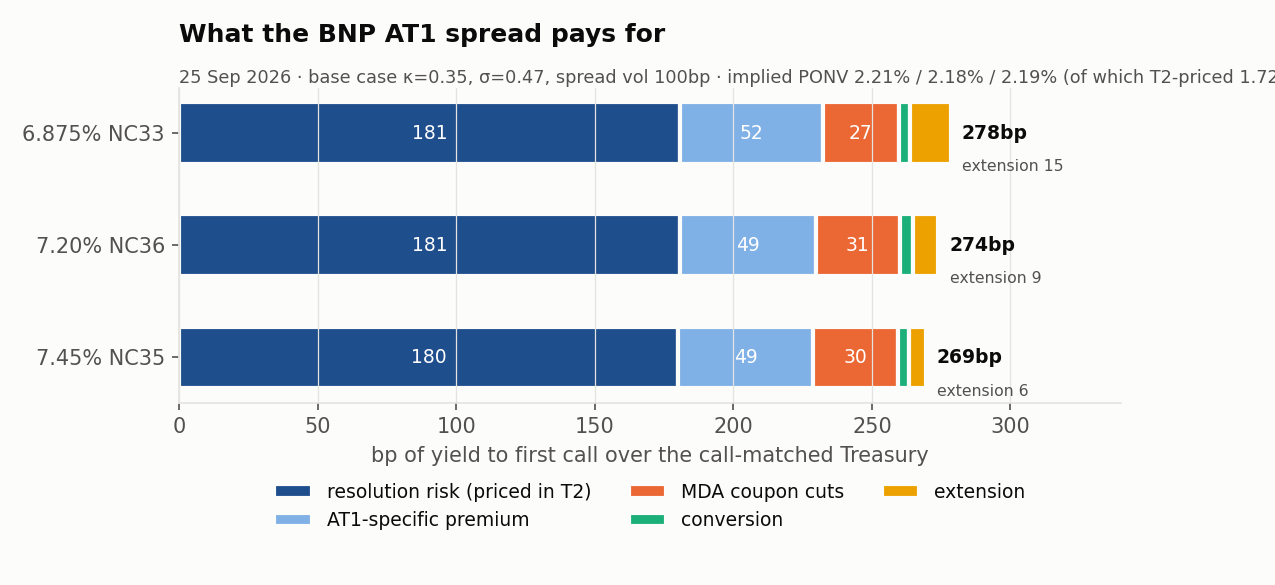
\includegraphics[width=0.88\textwidth]{spread_decomposition.png}
\caption{What the BNP AT1 spread pays for.}
\label{fig:decomp}
\end{figure}

Two-thirds of the spread, about $180$bp, is priced in Tier~2 as well. In the base case
another $50$bp is the premium for being an AT1 rather than a Tier~2: the risk of a write-down
without resolution, the equity-like, perpetual and discretionary profile, and the
instrument's liquidity. This component, unlike the first, depends on the speed of capital
mean reversion (Section~\ref{sec:uncert}). The contract features explain the rest. Expected MDA coupon cuts cost about $30$bp. Conversion
at the trigger, a $1.4$--$1.6\%$ lifetime event at a recovery of about a third, costs
$4$bp. Extension costs $6$--$15$bp and decreases with the reset margin, as it should: the
6.875\% has the lowest margin over today's AT1 spread and pays most for the issuer's option.

The MDA component is an upper bound, for the reasons given in Section~\ref{sec:institutions}:
the model applies the quartile factor to the coupon, while a bank inside its buffer would
cut dividends, buy-backs and variable pay first. Because the total spread is fixed by the
market price, an overstated MDA component is taken from the AT1-specific premium: given
$\kappa$, the $50$bp is a lower bound. Across values of $\kappa$ it is not. Slower capital
rebuilding raises the MDA and extension components and lowers the premium, which is close
to zero at the historical estimate of $\kappa$ (Table~\ref{tab:decompkappa}). What the
market price pins down is their sum with conversion: the $89$--$98$bp that each AT1 pays
over the Tier~2-priced risk.

\subsection{Call and extension}

\begin{table}[H]
\centering
\begin{tabular}{lccc}
\toprule
 & 6.875\% NC33 & 7.20\% NC36 & 7.45\% NC35 \\
\midrule
Reset margin $-$ today's AT1 spread (bp) & $+6$ & $+15$ & $+34$ \\
$\Pr(\text{called at }T_1)$ & 49\% & 52\% & 58\% \\
$\Pr(\text{called at some reset})$ & 97\% & 98\% & 98\% \\
Cost of the issuer's option (points) & 0.78 & 0.59 & 0.37 \\
P\&L if AT1 spreads settle $+50$bp (points) & $-3.3$ & $-3.5$ & $-3.2$ \\
\quad of which from extension (points) & $-1.2$ & $-0.9$ & $-0.7$ \\
\bottomrule
\end{tabular}
\caption{Call and extension. The cost of the option is the price if the call at $T_1$ were
certain minus the model price, at the same hazard. The extension P\&L is the extra loss
relative to a bond whose call at $T_1$ is certain.}
\label{tab:callext}
\end{table}

With a purely economic rule the first call is close to a coin toss, and almost certain at
some later reset. Figure~\ref{fig:calls} shows the probability of a call at the first reset
as a function of the long-run AT1 spread: at $200$bp all three bonds are called about three
times out of four, at $350$bp only a quarter to a third of the time. The low-margin 6.875\%
is always the least likely to be called and is the most negatively convex: if AT1 spreads
settle $50$bp wider, it loses $1.2$ points more than a bond with a certain call. The market
priced exactly this in September 2026: with the ten-year Treasury up 45bp in four weeks,
the 6.875\%'s spread widened by a further 34bp, against 10--12bp for the other two.

\begin{figure}[H]
\centering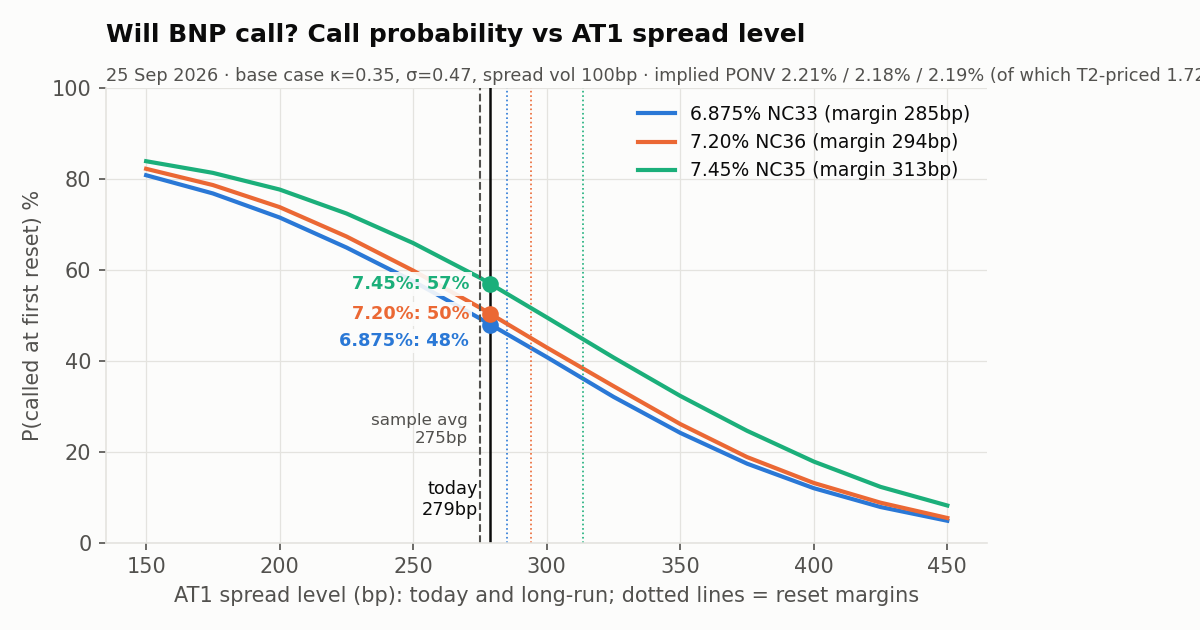
\includegraphics[width=0.8\textwidth]{call_probability.png}
\caption{Probability of a call at the first reset against the AT1 spread level, with
today's and the long-run spread both set to the value on the horizontal axis. Dots: base
case, with today's spread and the long-run level at the sample mean, as in
Table~\ref{tab:callext}.}
\label{fig:calls}
\end{figure}

\subsection{Stress and the capital cliff}

Each scenario of Table~\ref{tab:stress} reprices the bonds on the same random numbers. Rate
shocks move the discount rate and the reset reference; spread shocks move the current and
long-run AT1 spread and scale the hazard with it; capital shocks move today's CET1 ratio.
The two hazard shocks have market counterparts: doubling the Tier~2-priced hazard is roughly
what a doubling of BNP's Tier~2 spread would imply, and it costs three times as much as
doubling the AT1-specific premium.

\begin{table}[H]
\centering
\begin{tabular}{lccc}
\toprule
Clean price change (points) & 6.875\% NC33 & 7.20\% NC36 & 7.45\% NC35 \\
\midrule
Rates $+100$bp & $-5.3$ & $-6.4$ & $-6.1$ \\
Rates $-100$bp & $+5.7$ & $+7.0$ & $+6.7$ \\
CET1 $-2$pp & $-1.5$ & $-1.6$ & $-1.6$ \\
CET1 $-4.2$pp (EBA adverse) & $-9.8$ & $-11.1$ & $-10.4$ \\
AT1 spreads $+200$bp & $-16.4$ & $-16.2$ & $-15.4$ \\
Spreads $+200$bp, rates $-50$bp (March 2023 style) & $-14.5$ & $-13.8$ & $-13.0$ \\
EBA adverse $+$ spreads $+200$bp & $-25.4$ & $-26.6$ & $-25.1$ \\
Tier~2-priced hazard $\times2$ & $-11.9$ & $-13.0$ & $-12.3$ \\
AT1-specific premium $\times2$ & $-3.6$ & $-3.8$ & $-3.6$ \\
\bottomrule
\end{tabular}
\caption{Stress scenarios, base case.}
\label{tab:stress}
\end{table}

\begin{table}[H]
\centering
\begin{tabular}{lcccccc}
\toprule
CET1 level & 13\% (today) & 12\% & 11\% & 10.5\% & 9\% & 7\% \\
\midrule
6.875\% NC33 & 0.6 & 0.8 & 1.7 & 4.4 & 4.6 & 4.6 \\
7.45\% NC35 & 0.6 & 0.8 & 1.9 & 4.8 & 4.8 & 4.8 \\
\bottomrule
\end{tabular}
\caption{Capital delta: price points per $+1$pp of CET1, by CET1 level (finite differences
on a $0.5$pp grid).}
\label{tab:delta}
\end{table}

\begin{figure}[H]
\centering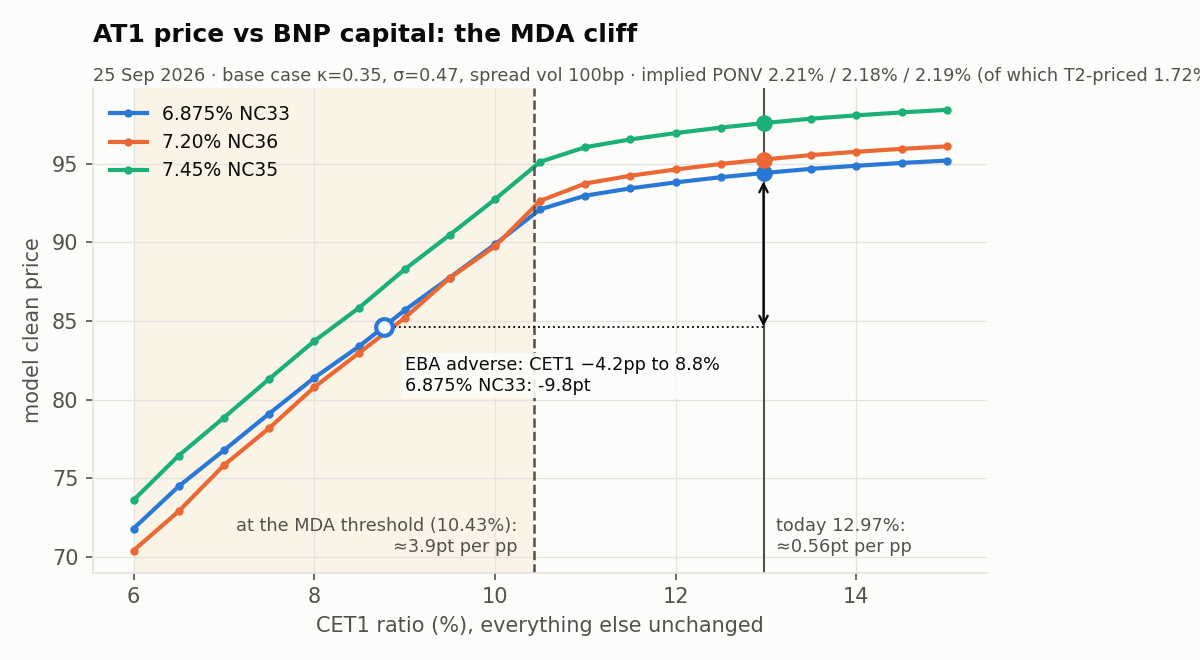
\includegraphics[width=0.8\textwidth]{price_vs_cet1.png}
\caption{Model price against today's CET1 ratio, everything else unchanged.}
\label{fig:cliff}
\end{figure}

Table~\ref{tab:delta} and Figure~\ref{fig:cliff} show the capital cliff. At today's ratio
the price moves by about $0.6$ points per point of CET1; within a point of the MDA threshold
the sensitivity rises to $4$--$5$ points. Crossing the threshold switches on three mechanisms
at once: coupons are cut by \eqref{eq:mda}, the call is blocked by \eqref{eq:call}, and the
hazard rises through \eqref{eq:seff}--\eqref{eq:hazard}. Because the O-SII step-ups raise the
threshold by 50bp by 2028, a capital loss of about half the EBA adverse depletion moves the
bonds from the flat part of the curve onto the cliff. The relevant risk measure for these
bonds is the distance to the MDA threshold, not the distance to the trigger.

\subsection{How much can we trust the capital parameters?}\label{sec:uncert}

Table~\ref{tab:kappa} reports the headline results, averaged across the three bonds, at the
two ends of the bootstrap interval for $\kappa$, at the maximum likelihood estimate and in the
base case. Each column recalibrates the implied hazards of the AT1s and, on the same paths,
the hazard of the Tier~2 anchor.

\begin{table}[H]
\centering
\begin{tabular}{lcccc}
\toprule
 & $\kappa=0.06$ & $\kappa=0.165$ & $\kappa=0.35$ & $\kappa=0.48$ \\
 & (5\%) & (MLE) & (base) & (95\%) \\
\midrule
Half-life of a capital shock (years) & 11.0 & 4.2 & 2.0 & 1.5 \\
Implied hazard (\%/yr) & 0.66 & 1.64 & 2.20 & 2.33 \\
\quad priced in Tier~2, $\lres$ (\%/yr) & 1.61 & 1.67 & 1.72 & 1.74 \\
\quad AT1-specific, $\lspec$ (\%/yr) & $-0.95$ & $-0.03$ & 0.47 & 0.59 \\
\quad Tier~2 share of the AT1 hazard & 244\% & 102\% & 78\% & 75\% \\
MDA coupon cost (points) & 14.5 & 6.3 & 2.5 & 1.7 \\
Capital delta at the MDA threshold (points/pp) & 13.7 & 8.8 & 4.2 & 2.8 \\
EBA adverse shock (points) & $-37.7$ & $-21.4$ & $-10.5$ & $-7.3$ \\
Cross-bond dispersion $D$ (bp) & 7.8 & 4.2 & 2.6 & 2.3 \\
\quad in price points & 0.6 & 0.3 & 0.2 & 0.2 \\
Log-likelihood relative to MLE & $-0.5$ & 0 & $-1.5$ & $-4.1$ \\
\bottomrule
\end{tabular}
\caption{Sensitivity to the speed of capital mean reversion (average of the three bonds).
$\lres$ is re-implied from the Tier~2 2035NC34 on the paths of each column. The capital
delta at the threshold is the central difference over $\pm0.25$pp.}
\label{tab:kappa}
\end{table}

\begin{figure}[H]
\centering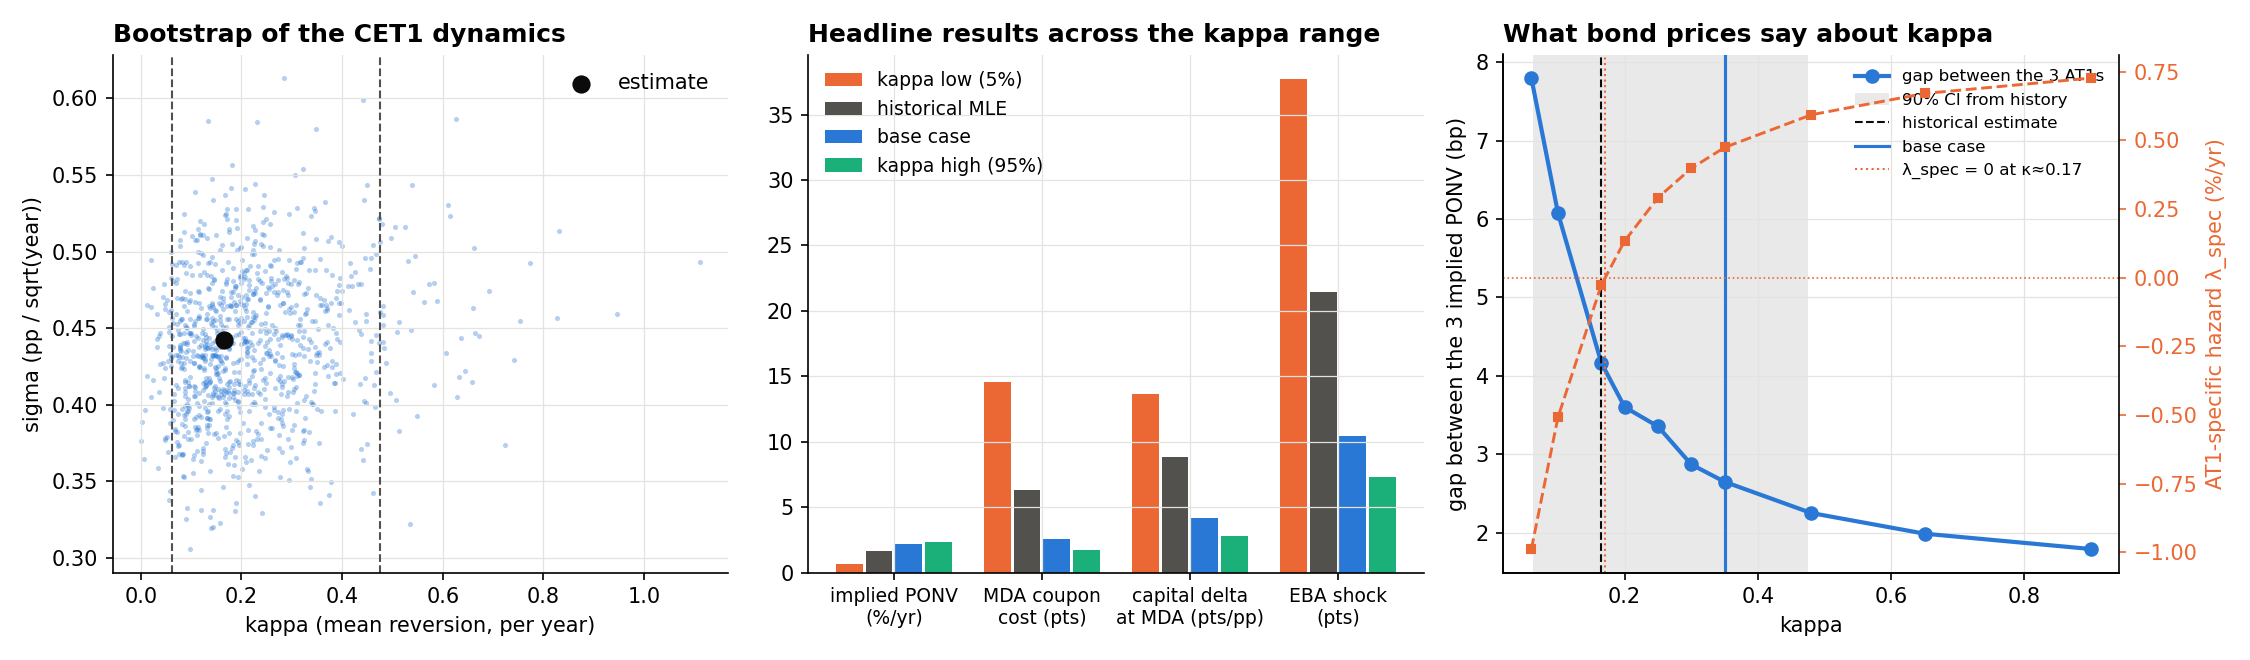
\includegraphics[width=\textwidth]{parameter_uncertainty.png}
\caption{Left: bootstrap of $(\kappa,\sigma)$. Centre: headline results across the
$\kappa$ range. Right: cross-bond dispersion of the implied hazard against $\kappa$ (left
axis) and the AT1-specific hazard $\lspec$ (right axis); the dotted line marks
$\lspec=0$.}
\label{fig:uncert}
\end{figure}

\paragraph{What prices add.} History and prices pull in opposite directions. The three
bonds are more consistent with fast capital rebuilding: the dispersion falls from $7.8$bp at
$\kappa=0.06$ to $2.3$bp at $0.48$ and then flattens. In price terms this is $0.6$ against
$0.2$ points, around the bid--offer, so the evidence is a lean, not an identification. The
history disfavours values much above $0.35$: the likelihood ratio statistic is $3.1$ at
$0.35$ and $8.1$ at $0.48$, and crosses the $5\%$ critical value of $3.84$ at about
$\kappa=0.37$.

\paragraph{What the Tier~2 adds.} The Tier~2 anchor gives a sharper restriction than the
cross-section of AT1s. Re-solved on the paths of each $\kappa$, the hazard priced in Tier~2
barely moves, from $1.61\%$ a year at $\kappa=0.06$ to $1.74\%$ at $\kappa=0.48$, so the
sensitivity to the capital dynamics falls almost entirely on the AT1-specific hazard. That
hazard is negative below $\kappa\approx0.17$: when capital is slow to rebuild, the model
attributes so much of the AT1's discount to expected MDA coupon cuts that the AT1 would be
priced as less risky than BNP's own Tier~2, which the creditor hierarchy rules out.
Requiring $\lspec\ge0$ excludes the lower half of the bootstrap interval and places the
bound at $\kappa=0.171$ for the average of the three bonds ($0.175$ for each bond
separately), a value that the history cannot distinguish from its maximum likelihood
estimate. Together with the likelihood, the admissible range is $\kappa\in[0.17,0.37]$, a
half-life of capital shocks between $1.9$ and $4.1$ years, over which $\lspec$ runs from zero
to about $0.49\%$ a year. The base case $\kappa=0.35$ lies in the upper part of this range,
where the cross-section of AT1s also points, and is consistent with BNP's active capital
management.

Table~\ref{tab:decompkappa} repeats the attribution of the spread at the two ends of the
admissible range, with $\sigma$, the AT1 hazards and the Tier~2 hazard re-solved for each
$\kappa$. The component priced in Tier~2 moves by less than half a basis point, and so does
the total that the AT1 pays over it. What moves is the split of that total. At
$\kappa=0.17$ the AT1-specific premium vanishes and its place is taken by expected coupon
cuts and by extension: with slow capital rebuilding, CET1 is more often below the MDA
threshold on a reset date, so the call is blocked more often and extension costs three
times as much as in the base case. Between $\kappa=0.35$ and $\kappa=0.37$ the attribution
hardly changes.

\begin{table}[H]
\centering
\begin{tabular}{lccc}
\toprule
bp of yield-to-call spread & $\kappa=0.171$ & $\kappa=0.35$ (base) & $\kappa=0.37$ \\
\midrule
Priced in Tier~2 (resolution) & 180.1 & 180.5 & 180.5 \\
AT1-specific premium & 1.0 & 49.8 & 52.3 \\
MDA coupon cuts & 52.0 & 29.4 & 27.9 \\
Conversion at the trigger & 6.7 & 4.3 & 4.1 \\
Extension & 34.0 & 10.0 & 9.1 \\
\midrule
AT1 over Tier~2 (premium and contract features) & 93.8 & 93.4 & 93.4 \\
Total $=$ market & 273.9 & 273.9 & 273.9 \\
\bottomrule
\end{tabular}
\caption{Attribution of the yield-to-call spread (base order, average of the three bonds)
at the ends of the range of $\kappa$ admitted by the CET1 history and the Tier~2
restriction, and in the base case. Each column re-solves $\sigma$, the AT1 hazards and the
Tier~2 hazard.}
\label{tab:decompkappa}
\end{table}

Two caveats qualify the bound. It is conditional on the stylised MDA rule: because
\eqref{eq:mda} overstates the expected coupon loss, and most so when capital is slow to
rebuild, the true bound lies below $0.17$. And $\lspec=0$ is the weakest restriction the
hierarchy imposes; any positive liquidity or equity premium on the AT1 would raise it.

\paragraph{Where the uncertainty sits.} With a slower mean reversion a capital shock lasts
longer, so more paths spend time inside the buffer: the MDA cost and the capital delta rise
and, since the total is fixed by the price, the implied hazard falls. Figure~\ref{fig:cliffunc}
re-calibrates each curve to today's price of the 6.875\%. All four agree at today's
$13\%$ CET1, and diverge only as capital falls: at the MDA threshold the price ranges from
$76$ ($\kappa=0.06$) to $93$ ($\kappa=0.48$), and at $6\%$ CET1 from $36$ to $77$. Bond prices
identify the level of risk today, not the shape of the cliff. What is robust across the
interval is the hazard priced in Tier~2, the ordering of the three bonds, the extension
ranking and the steepening of the capital delta near the threshold. The level of the
capital stress and the split of the AT1's excess over the Tier~2 among the AT1-specific
premium, the MDA component and extension are not; the Tier~2 restriction narrows their
range but does not remove it.

\begin{figure}[H]
\centering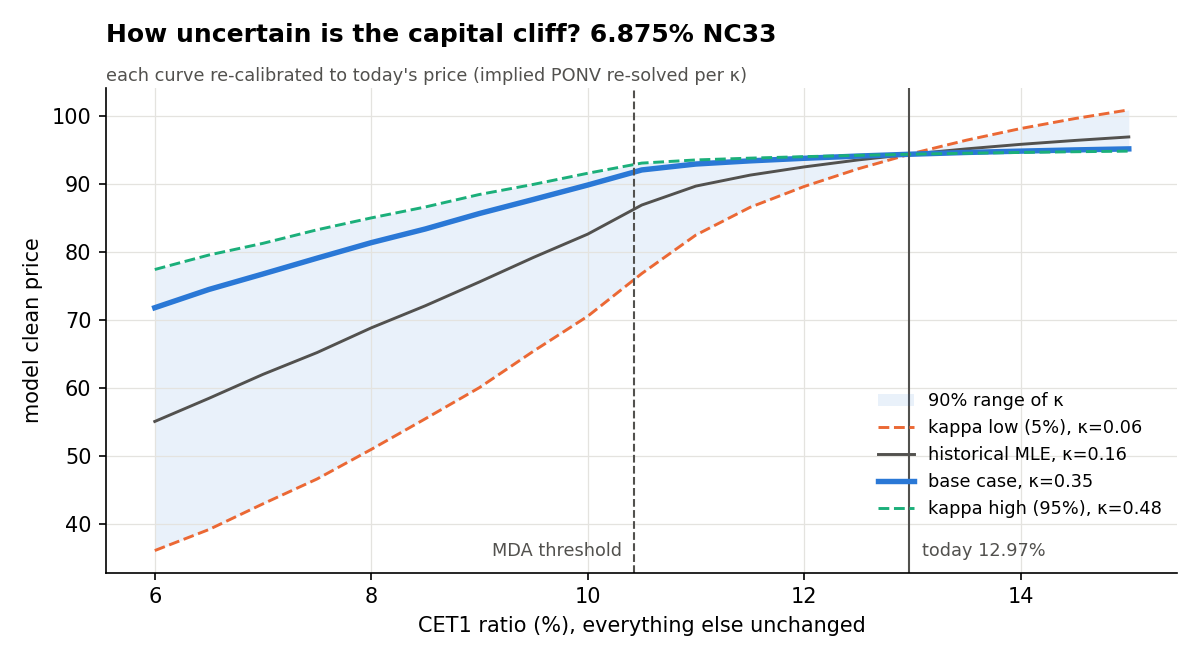
\includegraphics[width=0.8\textwidth]{capital_cliff_uncertainty.png}
\caption{Price of the 6.875\% NC33 against CET1 for four values of $\kappa$, each
re-calibrated to today's price. Shaded: $90\%$ bootstrap range of $\kappa$.}
\label{fig:cliffunc}
\end{figure}
%======================================================================
\section{Robustness}\label{sec:robust}
%======================================================================

This section asks whether the base-case split of the AT1 spread into about $180$bp priced
in Tier~2 and $50$bp of AT1-specific premium survives three objections a practitioner would
raise: that the call rule is unrealistic, that the attribution depends on the order of
features, and that a single flat resolution hazard is too crude for a perpetual. A fourth
objection, that the split depends on the weakly identified speed of capital mean reversion,
is treated in Section~\ref{sec:uncert}. It is the one the split does not fully survive: the
Tier~2-priced part is robust to it, the AT1-specific premium is not. All computations are on
the valuation date, on the same random numbers as the base case.

\subsection{Reputational calls}

The base call rule \eqref{eq:call} with $\delta=0$ calls only when refinancing is cheaper.
European national champions have almost always called their AT1s at the first opportunity,
and market participants quote call probabilities well above those of
Table~\ref{tab:callext}. We introduce a reputational tolerance: the issuer also calls when its
reset margin is up to $\delta$ \emph{below} the new-issue spread. For each $\delta$ we
recalibrate the hazard of each bond.

\begin{table}[H]
\centering
\begin{tabular}{lcccc}
\toprule
Tolerance $\delta$ (bp) & 0 & 25 & 50 & 100 \\
\midrule
$\Pr(\text{called at }T_1)$: 6.875\% NC33 & 49\% & 57\% & 65\% & 77\% \\
\phantom{$\Pr(\text{called at }T_1)$:} 7.20\% NC36 & 52\% & 60\% & 67\% & 79\% \\
\phantom{$\Pr(\text{called at }T_1)$:} 7.45\% NC35 & 58\% & 66\% & 72\% & 81\% \\
Implied hazard, 6.875\% (\%/yr) & 2.21 & 2.22 & 2.23 & 2.25 \\
Implied hazard, 7.20\% (\%/yr) & 2.18 & 2.19 & 2.20 & 2.21 \\
Implied hazard, 7.45\% (\%/yr) & 2.19 & 2.19 & 2.19 & 2.19 \\
Extension component, 6.875\% (bp) & 15 & 14 & 13 & 11 \\
Extension component, 7.20\% (bp) & 9 & 9 & 8 & 7 \\
Extension component, 7.45\% (bp) & 6 & 6 & 6 & 6 \\
Tier~2 share of the AT1 hazard & 78\% & 78\% & 78\% & 78\% \\
\bottomrule
\end{tabular}
\caption{Reputational call tolerance. The extension component is the yield-to-call spread of
the model price minus that of the same bond with a certain call at $T_1$.}
\label{tab:reputation}
\end{table}

A tolerance of $100$bp raises the probability of a call at the first reset to $77$--$81\%$,
the range practitioners quote, and lowers the extension component of the low-margin bond
from $15$ to $11$bp. The implied hazard moves by at most $4$bp, and the Tier~2 share of the
hazard does not move. The reason is that the market price pins down the total value of the
bond: a more generous call rule raises the value of the call leg slightly, and the hazard
adjusts to absorb it. The extension risk of the low-margin bond, and its negative convexity,
are therefore partly a feature of the economic call rule, while the split between Tier~2-priced
and AT1-specific risk is not.

\subsection{Order of attribution}

Table~\ref{tab:order} reports four attributions of the spread for each bond: the base order
(R, S, M, C, E), the nested Shapley value of Section~\ref{sec:attribution}, the full Shapley
value over all $120$ orders, and the reverse order (E, C, M, S, R).

\begin{table}[H]
\centering\small
\begin{tabular}{llcccc}
\toprule
Bond & Component & Base order & Nested Shapley & Full Shapley & Reverse order \\
\midrule
\multirow{5}{*}{6.875\% NC33} & Priced in Tier~2 & 180.7 & 180.8 & 221.1 & 259.1 \\
 & AT1-specific & 51.6 & 51.6 & 62.8 & 77.0 \\
 & MDA & 27.3 & 36.1 & 35.5 & 43.3 \\
 & Conversion & 4.1 & 5.5 & 6.4 & 11.7 \\
 & Extension & 14.7 & 4.5 & $-47.3$ & $-112.6$ \\
\midrule
\multirow{5}{*}{7.20\% NC36} & Priced in Tier~2 & 180.8 & 180.9 & 206.9 & 231.4 \\
 & AT1-specific & 48.8 & 48.8 & 55.7 & 64.4 \\
 & MDA & 30.6 & 36.0 & 35.1 & 39.3 \\
 & Conversion & 4.6 & 6.0 & 6.8 & 11.0 \\
 & Extension & 9.1 & 2.4 & $-30.4$ & $-72.0$ \\
\midrule
\multirow{5}{*}{7.45\% NC35} & Priced in Tier~2 & 180.0 & 180.0 & 203.6 & 225.9 \\
 & AT1-specific & 48.9 & 48.8 & 55.1 & 62.9 \\
 & MDA & 30.4 & 35.8 & 35.0 & 39.2 \\
 & Conversion & 4.0 & 5.3 & 6.1 & 10.1 \\
 & Extension & 6.0 & $-0.6$ & $-30.4$ & $-68.8$ \\
\bottomrule
\end{tabular}
\caption{Attribution of the yield-to-call spread (bp) under four methods. Totals are
$278.5$, $274.0$ and $269.3$bp in every column.}
\label{tab:order}
\end{table}

Three conclusions follow.

\emph{First}, the split of the hazard block is order-free. In every attribution that prices
the hazard before the contract features, the base order and the nested Shapley value, the
Tier~2-priced and AT1-specific components agree to within $0.2$bp. This is the near-linearity
of Proposition~\ref{prop:hazardsplit}: on the relevant range the yield-to-call spread is
almost linear in the hazard level, so it does not matter in which order $\lres$ and $\lspec$
are switched on.

\emph{Second}, the attribution among the contract features is order-dependent. Their total
is the same in the base order and in the nested value ($40$--$46$bp depending on the bond),
but its split is not: symmetric treatment raises the MDA component to about $36$bp and
reduces extension to a few basis points. The two features interact through the capital
condition of the call rule. The states in which the call is blocked because CET1 is below the
threshold are the states in which the MDA cuts coupons; once the MDA is priced, the
cash flows of the bond in those states are already reduced, so the incremental cost of not
being called is smaller, and conversely. The honest statement is that the contract features
cost $40$--$46$bp, of which MDA is $27$--$36$bp, conversion $4$--$6$bp and extension between
$-1$ and $15$bp.

\emph{Third}, orders that switch extension on before the hazard produce economically
meaningless results. Without any hazard, the bond is risk-free, and not calling a risk-free
bond that pays its reset margin over Treasuries is a gift to the investor: extension takes a
large negative value ($-69$ to $-113$bp in the reverse order) and the hazard components absorb
the difference. This is the inconsistency the state-dependent hazard is designed to avoid
(Section~\ref{sec:hazard}); it shows why the full Shapley value, which averages over such orders,
is the wrong benchmark for AT1 attribution.

\subsection{Term structure of the resolution hazard}

A single flat $\lres$, calibrated to a bond with a 2034 call, is applied to AT1 cash flows
that run for decades if the bond is extended. With the two Tier~2 bonds we bootstrap a
two-piece resolution hazard as in Section~\ref{sec:piecewise}.

\begin{table}[H]
\centering
\begin{tabular}{lccc}
\toprule
 & 6.875\% NC33 & 7.20\% NC36 & 7.45\% NC35 \\
\midrule
$\lambda_1$ to August 2030 (\%/yr) & 1.40 & 1.40 & 1.40 \\
$\lambda_2$ after August 2030 (\%/yr) & 2.10 & 2.10 & 2.10 \\
Flat $\lres$ (\%/yr) & 1.72 & 1.72 & 1.72 \\
$\lspec$, flat $\lres$ (\%/yr) & 0.49 & 0.46 & 0.47 \\
$\lspec$, two-piece $\lres$ (\%/yr) & 0.42 & 0.36 & 0.39 \\
Tier~2-priced component, flat (bp) & 180.7 & 180.8 & 180.0 \\
Tier~2-priced component, two-piece (bp) & 176.4 & 184.6 & 181.2 \\
\bottomrule
\end{tabular}
\caption{Two-piece resolution hazard bootstrapped from the Tier~2 2035NC30 (call August 2030)
and the Tier~2 2035NC34 (call November 2034), recovery $20\%$.}
\label{tab:termstructure}
\end{table}

The resolution hazard is upward sloping: $1.40\%$ a year to 2030 and $2.10\%$ after. With
the steeper curve, more of each AT1's hazard is attributed to what Tier~2 prices, and the
AT1-specific hazard falls from $0.47\%$ to $0.39\%$ on average. The Tier~2-priced component
of the spread moves by less than $5$bp, in different directions for different bonds
depending on the timing of their cash flows. A term structure therefore strengthens, rather
than weakens, the conclusion that most of the AT1 spread is priced in Tier~2. A caveat
applies to the short Tier~2: it trades well below par with a reset in 2030, and its price
may contain a convexity or tax effect that a bullet-to-call treatment ignores.
%======================================================================
\section{Discussion}\label{sec:discussion}
%======================================================================

\subsection{What the AT1-specific premium is}

The AT1-specific hazard, $0.4$--$0.5\%$ a year in the base case, about $50$bp of spread, is
the part of the AT1's compensation that BNP's Tier~2 does not earn and that the model's MDA
rule does not explain. Proposition~\ref{prop:clocks} gives it a
precise risk-neutral meaning: it is the intensity of write-downs that hit the AT1 without a
resolution that also hits Tier~2, plus whatever premium investors attach to the instrument
beyond its expected loss. Four components are plausible, and the model cannot separate them.
\begin{enumerate}
  \item \emph{Write-down without resolution.} The Credit Suisse case showed that AT1 holders
  can lose everything in a transaction that leaves more junior or more senior claims
  partially intact. The EU authorities' March 2023 statement makes this less likely in the
  EU, but it does not make it impossible, and investors price the tail.
  \item \emph{Coupon discretion beyond the MDA.} The issuer may cancel coupons for reasons
  other than the MDA, and supervisors can restrict distributions outside the MDA rule, as
  they did with dividends in 2020. The model's MDA rule does not capture this.
  \item \emph{Equity-like risk premium.} An AT1 bond is perpetual, its payoff in bad states is
  close to that of equity, and its investor base includes funds with mandates that force
  sales in stress. The premium for bearing this risk need not be the same as Tier~2's.
  \item \emph{Liquidity.} AT1 bonds trade with wider bid--offer spreads than Tier~2 and are
  excluded from some benchmark indices.
\end{enumerate}
Because the MDA component is an upper bound, the $50$bp is a lower bound for these four
together, given the speed of capital mean reversion. It is not a lower bound across values
of that speed. With slower capital rebuilding, the model assigns more of the AT1's discount
to expected MDA coupon cuts and to extension and less to these four components, and at the
historical estimate it assigns them nothing (Table~\ref{tab:decompkappa}). What the data
identify is the total that the AT1 pays over the Tier~2-priced risk, $89$--$98$bp, which
does not move with the capital dynamics; its split rests on the capital dynamics and on
the MDA rule, the two weakest parts of the model.

\subsection{Implications}

\paragraph{For investors.} Two-thirds of an AT1's spread is compensation that the same
issuer's Tier~2 also pays, at a better recovery and without extension or coupon risk. The
relevant relative-value question is therefore whether the remaining $89$--$98$bp, the
AT1-specific premium together with the contract features, is adequate compensation for
those features, not whether $275$bp is a high spread in absolute terms. That total is
better determined than its parts. The model provides a consistent way to
make that comparison across issuers: calibrate $\lres$ to each issuer's Tier~2 and compare the
residuals.

\paragraph{For risk management.} The price is flat in capital at today's level and steep
within a point of the MDA threshold. A risk system that measures the distance to the trigger
will understate the capital risk of these bonds; the relevant distance is to the threshold,
which itself moves with scheduled buffer changes. The capital delta at the threshold is
three to eight times the delta today, depending on the speed of capital mean reversion
(Table~\ref{tab:kappa}).

\paragraph{For the extension decision.} The low-margin bond is the most exposed to extension
under an economic call rule, and the market behaved accordingly in September 2026. Whether
the issuer would in fact extend is a question about its reputational incentives; the
robustness results show that this question affects the extension component of the spread,
but not the hazard or its split.

\subsection{Limitations}

\begin{enumerate}
  \item \textbf{Measure.} CET1 dynamics are estimated under the physical measure and assumed
  to hold under the pricing measure. All residual premia are in $\lambda$, which is a
  risk-neutral intensity. The Tier~2 anchor splits it, but $\lres$ is risk-neutral too and
  contains Tier~2's own premia.
  \item \textbf{Recovery.} The split depends on the Tier~2 recovery (Table~\ref{tab:recovery}).
  The market prices are consistent with the conventional $20\%$, but recovery is not observed.
  \item \textbf{Capital mean reversion.} $\kappa$ is weakly identified by history, and the
  capital stress results scale by a factor of five across its bootstrap interval. The
  Tier~2 restriction $\lspec\ge0$ excludes the lower half of that interval and reduces the
  factor to about two, but it is itself conditional on the stylised MDA rule. The
  AT1-specific premium depends on $\kappa$; the Tier~2-priced hazard does not.
  \item \textbf{MDA mechanics.} Applying the quartile factor to the coupon overstates the MDA
  cost. The leverage-ratio and MREL MDAs, the available distributable items and supervisory
  discretion over distributions are not modelled.
  \item \textbf{Call behaviour.} The base rule is economic; a reputational tolerance changes
  the call probabilities but not the hazard. The regulatory approval test of CRR
  Art.~77--78 is approximated by the MDA threshold.
  \item \textbf{No systemic or sovereign factor.} The spread process is issuer-specific and
  capital jumps do not move spreads. AT1 spreads widened by hundreds of basis points in March
  2020 and March 2023 with no change in capital, and BNP's spreads widened with French
  sovereign stress after the valuation date. A common sector and sovereign factor with
  co-jumps in capital and spreads is the main extension.
  \item \textbf{Rates.} The current curve is used for all future resets; a short-rate model
  would add rate-driven extension.
  \item \textbf{Unidentified spread parameters.} The spread volatility $\eta$ and the capital
  premium $\beta$ are assumed. A cross-section of issuers, or a regression of AT1 spreads on the
  distance to the MDA threshold, would calibrate $\beta$.
  \item \textbf{Data.} Prices are evaluated rather than traded; the sample covers fifteen
  months of relatively tight spreads; the bid--offer is of the same size as the cross-bond
  dispersion; the CDS is in EUR and the bonds in USD. TRACE transaction prices would allow a
  test on traded data.
  \item \textbf{Conversion.} A single stressed share price replaces a joint model of equity and
  capital; with conversion worth $4$bp this is immaterial for BNP, but not for an issuer close
  to its trigger.
\end{enumerate}

\subsection{Extensions}

Three extensions follow naturally. A common factor in spreads and capital, estimated on a
cross-section of European AT1 issuers, would capture the systemic component of the risk and
allow the AT1-specific premium to be decomposed into issuer and sector parts. A model of
distributions in which the bank allocates the MDA between dividends and coupons would
replace the upper bound on the MDA cost by an estimate. And a joint calibration across
issuers, with $\lres$ anchored to each issuer's Tier~2, would turn the residual premium into a
relative-value signal.

%======================================================================
\section{Conclusion}\label{sec:conclusion}
%======================================================================

AT1 bonds are claims on bank capital, and modelling them as such makes their three main
contingencies, the trigger, the coupon restriction and the call, consistent by construction.
Capital alone cannot explain their prices: the model needs a refinancing spread that drives
the call and a write-down hazard that rises in the same states. Conditioning on the state
paths makes the price an explicit, smooth and convex function of the hazard, so the implied
hazard is unique and every comparative static is exact on a given set of paths.

The implied hazard is not a black box. Because Tier~2 faces the same resolution event as AT1,
pricing the issuer's Tier~2 on the same state splits the hazard into a part Tier~2 also
prices and an AT1-specific premium. For BNP Paribas in September 2026, about two-thirds of
the spread, some $180$bp, is priced in Tier~2 as well. This part survives a reputational
call rule, every attribution that prices the hazard before the contract features, a term
structure of the resolution hazard and the range of capital dynamics that history and the
Tier~2 jointly admit. The remaining $89$--$98$bp pays for being an AT1 rather than a Tier~2, and is
equally robust. How it divides among expected MDA coupon cuts, extension and an
AT1-specific premium depends on how fast the bank rebuilds capital after a shock: the
premium is about $50$bp in the base case and zero at the historical estimate. The same dependence drives the level of the capital
stress. The Tier~2 narrows both, because the creditor hierarchy forbids pricing the AT1 as
safer than the Tier~2, but it does not remove them, and both are reported with their
range.

\appendix
%======================================================================
\section{Further derivations}\label{app:derivations}
%======================================================================

\subsection{Isometry for the compound Poisson integral}

Let $\tilde L_t=L_t-\lambda_Jm_Jt$ be the compensated compound Poisson process. For a
deterministic square-integrable $f$, $\E\int_0^tf(u)\dd\tilde L_u=0$ and
\[
  \E\Bigl[\Bigl(\int_0^tf(u)\dd\tilde L_u\Bigr)^2\Bigr]=\lambda_J\E[J^2]\int_0^tf(u)^2\dd u .
\]
\emph{Proof.} For a step function $f=\sum_kf_k\1_{(u_k,u_{k+1}]}$ the increments of $\tilde L$
over disjoint intervals are independent with mean zero and variance
$\lambda_J\E[J^2](u_{k+1}-u_k)$, so the second moment is
$\lambda_J\E[J^2]\sum_kf_k^2(u_{k+1}-u_k)$. The general case follows by density of step
functions in $L^2$. Writing $\int f\dd L=\int f\dd\tilde L+\lambda_Jm_J\int f\dd u$ gives the mean
and variance used in Proposition~\ref{prop:cet1}, with $f(u)=e^{-\kappa(t-u)}$.

\subsection{Transition of the CET1 process between observation dates}

Conditionally on $C_s$, \eqref{eq:cet1sol} applied on $[s,t]$ gives
\[
  C_t=\theta+(C_s-\theta)e^{-\kappa(t-s)}+\sigma\int_s^te^{-\kappa(t-u)}\dd W_u-\int_s^te^{-\kappa(t-u)}\dd L_u .
\]
Without jumps the transition is Gaussian with mean $m=\theta+(C_s-\theta)e^{-\kappa\Delta}$ and
variance $\sigma^2(1-e^{-2\kappa\Delta})/(2\kappa)$, $\Delta=t-s$, which is \eqref{eq:outrans}.
With jumps it is a Gaussian mixture: conditionally on $k$ jumps at times
$u_1,\dots,u_k$, the mean is shifted by $-\sum_iJ_ie^{-\kappa(t-u_i)}$. The likelihood used in
Section~\ref{sec:calibration} ignores this term. Over a quarter the probability of a jump is
$1-e^{-0.12/4}\approx3\%$, so the Gaussian likelihood treats rare large moves as diffusion,
which biases $\hat\sigma$ upwards slightly and, through the profile likelihood, $\hat\kappa$ in
an ambiguous direction; the 2023Q1 exclusion removes the one large positive move.

\subsection{Profile likelihood}

Differentiating \eqref{eq:loglik} with respect to $\sigma^2$ gives
$\partial\ell/\partial\sigma^2=-\frac{n}{2\sigma^2}+\frac1{2\sigma^4}\sum_k(C_{k+1}-m_k)^2/w_k$,
which vanishes at \eqref{eq:sigmahat}. Substituting back,
\[
  \ell_p(\kappa)=\ell\bigl(\kappa,\hat\sigma(\kappa)\bigr)
  =-\frac n2\Bigl[1+\log\bigl(2\pi\hat\sigma^2(\kappa)\bigr)\Bigr]-\frac12\sum_k\log w_k(\kappa),
\]
a one-dimensional function of $\kappa$. The likelihood ratio statistic for a fixed $\kappa_0$
is $2[\ell_p(\hat\kappa)-\ell_p(\kappa_0)]$, asymptotically $\chi^2_1$.

\subsection{Yield to call and the delta method}

Let $y(V)$ solve $V=\sum_jc_j(1+y/2)^{-2t_j}$ for the bullet cash flows $c_j$ to $T_1$. By the
implicit function theorem
\[
  \frac{\dd y}{\dd V}=-\Bigl[\sum_jc_jt_j(1+y/2)^{-2t_j-1}\Bigr]^{-1}=-\frac{1}{D_{\mathrm{mod}}V},
\]
where $D_{\mathrm{mod}}$ is the modified duration to call. For a zero-recovery bullet to
$T_1$ with a constant hazard $h$, the price is the risk-free price discounted at $r+h$, so the
continuously compounded yield rises one-for-one with the hazard; in the base attribution the
hazard block of $219$bp of hazard produces $231$bp of semi-annual yield-to-call spread, a ratio
of $1.05$ that reflects compounding and the state dependence of the driver. The price
sensitivity $|V_0'|\approx0.08$ points per basis point of hazard is larger than a bullet's,
because it includes the exposure of extended cash flows beyond $T_1$. The delta method for the
implied hazard, \eqref{eq:sehazard}, follows from the same implicit function argument applied
to $V_0(\lambda)=P$.

\subsection{The credit triangle for the CDS reference points}

For a CDS with constant hazard $h$, recovery $R$ and continuous premium $s$, the protection
leg is $(1-R)\int_0^Th e^{-(r+h)u}\dd u$ and the premium leg $s\int_0^Te^{-(r+h)u}\dd u$, so the
par spread is $s=h(1-R)$ and $h=s/(1-R)$. The CDS rows of Table~\ref{tab:ladder} use this
approximation; it ignores the term structure of the hazard, accrued premium on default and
the difference between the standard coupon and the par spread, all of which are small at
these spread levels.

\subsection{Relation of the nested value to the Owen value}

For a game $v$ on $\mathcal N$ with a partition into unions $\{\mathcal H,\mathcal K\}$, the
Owen value of player $j\in\mathcal H$ averages its marginal contribution over all orders in
which the members of each union are contiguous, with both orders of the unions equally
likely \citep{Owen1977}. The nested value of Section~\ref{sec:attribution} restricts these
orders to those in which $\mathcal H$ comes first. It is therefore the Owen value of the game
in which the union order is fixed, and it inherits efficiency, symmetry within unions and
the null-player property. The full Owen value would average the nested value with the
attribution in which the contract block comes first, which values extension on a riskless
bond and is excluded for the reason given in Section~\ref{sec:robust}.


%======================================================================
\section{Numerical diagnostics}\label{app:numerics}
%======================================================================

\paragraph{Monte Carlo error.} Table~\ref{tab:mcerr} reports, for each AT1 on the valuation
date, the path-wise standard deviation of the conditional payoff, the standard error of the
price with $20{,}000$ paths, the sensitivity of the price to the hazard and the implied
standard error of the hazard from \eqref{eq:sehazard}.

\begin{table}[H]
\centering
\begin{tabular}{lccc}
\toprule
 & 6.875\% NC33 & 7.20\% NC36 & 7.45\% NC35 \\
\midrule
Path-wise s.d.\ of conditional payoff (points) & 7.3 & 7.9 & 7.5 \\
Standard error of the price (points) & 0.051 & 0.056 & 0.053 \\
$|\partial V/\partial\lambda|$ (points per bp) & 0.077 & 0.084 & 0.079 \\
Standard error of $\lambda$ (bp) & 0.67 & 0.66 & 0.67 \\
\bottomrule
\end{tabular}
\caption{Monte Carlo error at the implied hazard, $20{,}000$ paths.}
\label{tab:mcerr}
\end{table}

\paragraph{Convergence.} Table~\ref{tab:conv} reports the implied hazards for path counts from
$5{,}000$ to $40{,}000$ with two independent seeds, and for a fortnightly instead of a
monthly grid. The levels vary by about $\pm1$bp across seeds, in line with the standard
errors of Table~\ref{tab:mcerr}. The cross-bond dispersion is much more stable, at
$2.3$--$2.9$bp across all runs, because the three bonds share their random numbers.
Halving the time step changes the hazards by at most $1.6$bp.

\begin{table}[H]
\centering
\begin{tabular}{llccc}
\toprule
Paths & Seed & 6.875\% NC33 & 7.20\% NC36 & 7.45\% NC35 \\
\midrule
5,000 & 11 & 2.213 & 2.193 & 2.196 \\
5,000 & 23 & 2.215 & 2.183 & 2.195 \\
10,000 & 11 & 2.215 & 2.191 & 2.196 \\
10,000 & 23 & 2.216 & 2.195 & 2.201 \\
20,000 & 11 & 2.210 & 2.186 & 2.188 \\
20,000 & 23 & 2.199 & 2.176 & 2.176 \\
40,000 & 11 & 2.215 & 2.184 & 2.190 \\
40,000 & 23 & 2.201 & 2.176 & 2.180 \\
\midrule
20,000, monthly (base) & 7 & 2.211 & 2.185 & 2.187 \\
20,000, fortnightly & 7 & 2.227 & 2.196 & 2.181 \\
\bottomrule
\end{tabular}
\caption{Implied hazards (\%/yr) by number of paths, seed and time step.}
\label{tab:conv}
\end{table}

\paragraph{Analytic moments.} With the base-case parameters,
Proposition~\ref{prop:cet1} gives a stationary CET1 mean of $12.25\%$ and a stationary
standard deviation of $1.17$pp ($0.56$pp from the diffusion alone); the mean jump is $2.2$pp
and its $95$th percentile $4.4$pp. Proposition~\ref{prop:spread} gives a stationary spread
standard deviation of $100$bp and a stationary probability of a negative spread of $0.3\%$.
The half-lives of shocks are $2.0$ years for capital and $1.4$ years for the spread.

\paragraph{Memory.} The conditional estimator stores, per path, the coupon cash flows and the
integrated driver at the coupon dates. Root-finding with closures over these arrays creates
reference cycles that the Python garbage collector does not free promptly; forcing a
collection after each solve keeps the weekly calibration below 1~GB.

%======================================================================
\section{Parameters}\label{app:params}
%======================================================================

\begin{table}[H]
\centering\small
\begin{tabular}{llll}
\toprule
Symbol & Meaning & Value & Source \\
\midrule
$\theta$ & CET1 target & 13\% & BNP strategic plan \\
$\kappa,\sigma$ & CET1 mean reversion, volatility & 0.35, 0.47pp & base case; MLE 0.165, 0.44 \\
$\lambda_J,m_J,\sigma_J$ & stress jumps & 0.12/yr, 2.2pp, 0.5 & EBA 2025 adverse check \\
$b$ & MDA floor & 5.64\% & P1 + P2R (CET1 part) \\
$w_0$ & combined buffer today & 4.79\% & published requirement 10.43\% \\
$\Delta w$ & O-SII step-ups & +0.25pp, 1-Jan-2027 and 2028 & French O-SII framework \\
$\ctrig$ & trigger & 5.125\% & term sheets \\
$a,\bar s,\eta,\rho$ & spread OU & 0.5, 275bp, 100bp, $-0.3$ & sample mean; assumptions \\
$\beta$ & capital premium & 1\% per pp & assumption \\
$\delta$ & reputational tolerance & 0 (base), up to 100bp & Section~\ref{sec:robust} \\
$\xi$ & share price at trigger / today & 0.2 & assumption \\
$R_{\mathrm{T2}},R_{\mathrm{SNP}}$ & recovery at resolution & 20\%, 40\% & Markit conventions \\
$\lambda$ & AT1 hazard today & 2.19\% (average) & implied \\
$\lres$ & hazard priced in Tier~2 & 1.72\% & implied, T2 2035NC34 \\
$\lambda_1,\lambda_2$ & two-piece $\lres$ & 1.40\%, 2.10\% & implied, both Tier~2 \\
$H,\Delta,n$ & horizon, step, paths & 40 years, 1/12, 20,000 & numerical \\
\bottomrule
\end{tabular}
\caption{Parameters of the base case.}
\end{table}

%======================================================================
\section{Data and reproducibility}\label{app:data}
%======================================================================

\paragraph{Data layout.} The repository separates raw Capital IQ exports
(\texttt{data/raw/}, licensed and not redistributed), public reference inputs
(\texttt{data/reference/}: term sheets, the requirement stack and its sources, the EBA stress
test and the FRED curve) and the processed panel built from them (\texttt{data/processed/}).
A single script, \texttt{build\_bnp\_dataset.py}, produces a daily panel of all six bonds with
accrued interest, yield to first call and spread over the FRED curve, together with the CDS,
the share price and the CET1 print available on each date, and a quarterly capital table
with the requirement and its publication date.

\paragraph{Code map.}
\begin{center}
\small
\begin{tabular}{ll}
\toprule
File & Content \\
\midrule
\texttt{processes.py} & CET1 jump-diffusion \eqref{eq:cet1}, trigger times \\
\texttt{instrument.py} & MDA schedule \eqref{eq:mda}, stylised term sheet \\
\texttt{market.py} & dated bonds, \eqref{eq:spread}--\eqref{eq:hazard}, pricing \eqref{eq:cmc},
  implied $\lambda$; Tier~2 \eqref{eq:t2grid}; piecewise hazard \\
\texttt{data.py} & paths, loaders, valuation date \\
\texttt{build\_bnp\_dataset.py} & raw exports to the processed panel \\
\texttt{calibrate\_bnp.py} & CET1 likelihood, weekly implied hazards, cross-section \\
\texttt{capital\_structure.py} & Tier~2/SNP/CDS ladder, recovery sensitivity, weekly split \\
\texttt{spread\_and\_stress.py} & attribution, call analysis, stress, capital delta \\
\texttt{robustness.py} & reputational call, Shapley attributions, term structure \\
\texttt{parameter\_uncertainty.py} & bootstrap of $(\kappa,\sigma)$, $\kappa$ scan \\
\texttt{numerics.py} & Monte Carlo errors, convergence, analytic moments \\
\bottomrule
\end{tabular}
\end{center}

\paragraph{Reproduction.} \texttt{run\_all.sh} rebuilds the panel, runs the test suite
(32 tests, including the reduction of the piecewise hazard to the flat one, the
round trip of the implied resolution hazard and the effect of the call tolerance), and
regenerates every table and figure in about thirty minutes. Dates, levels and annotations in
the figures are read from the data, so newer exports and a new \texttt{VALUATION\_DATE}
update the whole paper.

%======================================================================
\section{Additional figures}\label{app:figures}
%======================================================================

\begin{figure}[H]
\centering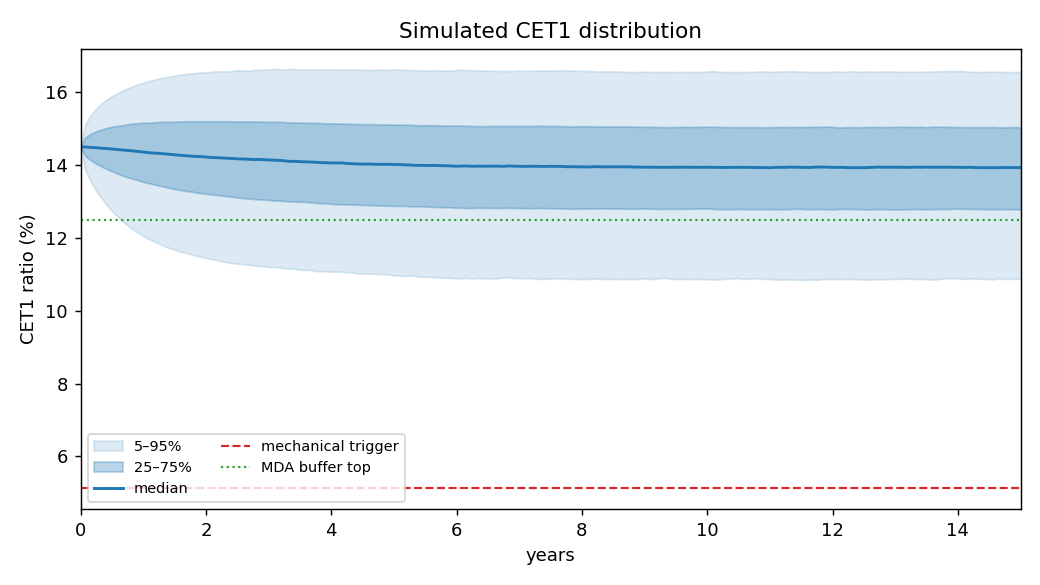
\includegraphics[width=0.75\textwidth]{cet1_fan_chart.png}
\caption{The stylised engine of the repository with illustrative parameters (not the BNP
calibration): simulated CET1 distribution over fifteen years, with the top of the MDA buffer
and the mechanical trigger.}
\end{figure}

\begin{figure}[H]
\centering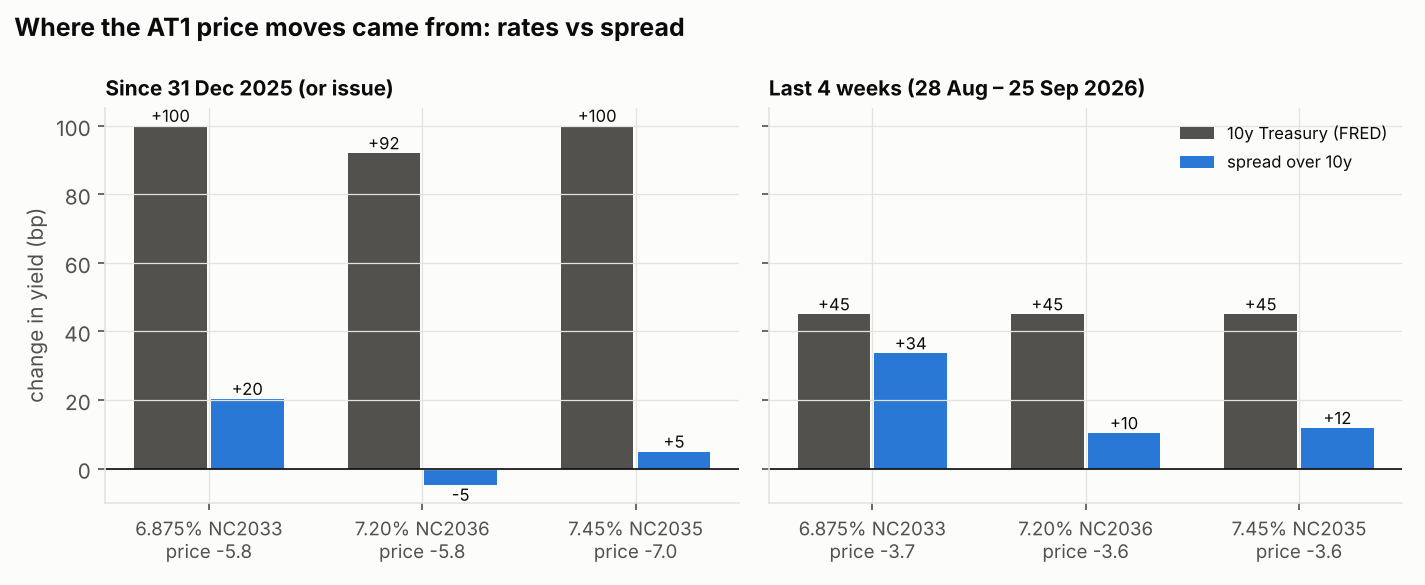
\includegraphics[width=0.85\textwidth]{bnp_at1_yield_split.png}
\caption{Change in each AT1's yield since 31 December 2025 (or issue) and over the four weeks
to 25 September 2026, split into the change in the ten-year Treasury yield and the change in
the spread over it.}
\end{figure}

\begin{figure}[H]
\centering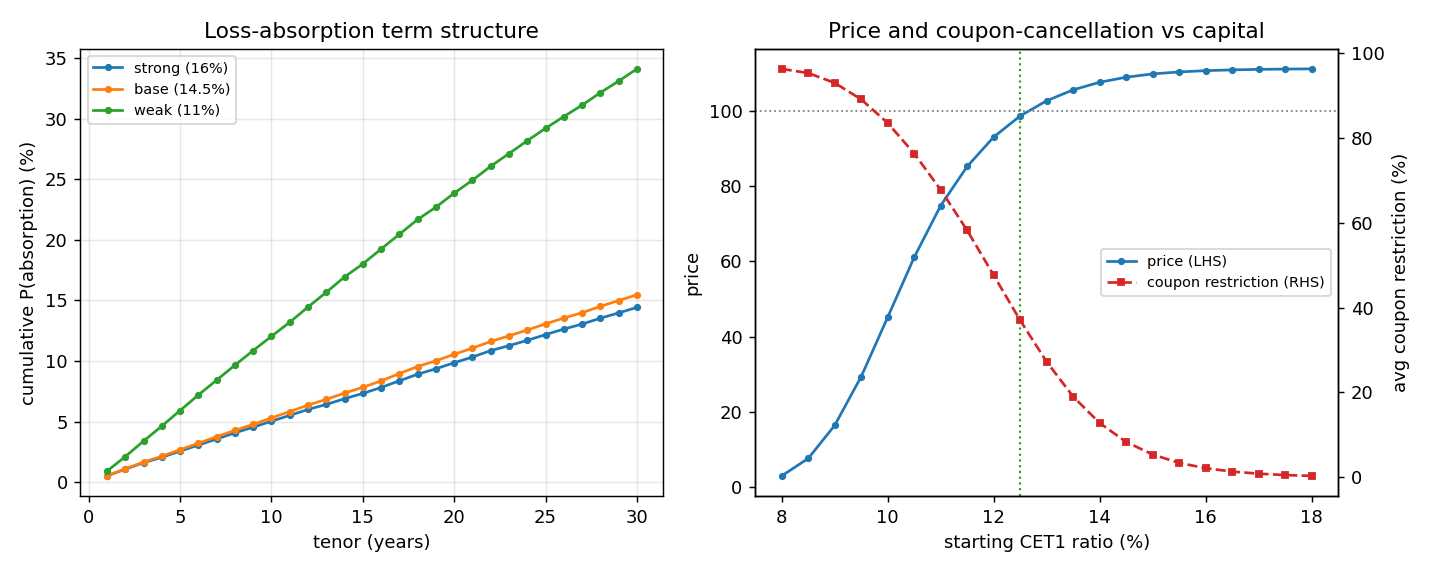
\includegraphics[width=0.85\textwidth]{absorption_and_price_curves.png}
\caption{The stylised engine with illustrative parameters: cumulative probability of loss
absorption by tenor for a strong, base and weak bank (left), and price and average coupon
restriction against the starting CET1 ratio (right).}
\end{figure}


%======================================================================
\begin{thebibliography}{99}
\addcontentsline{toc}{section}{References}

\bibitem[Avdjiev et~al.(2013)]{AvdjievEtAl2013}
Avdjiev, S., Kartasheva, A. and Bogdanova, B. (2013).
\newblock CoCos: a primer.
\newblock \emph{BIS Quarterly Review}, September, 43--56.

\bibitem[Bielecki and Rutkowski(2002)]{BieleckiRutkowski2002}
Bielecki, T.~R. and Rutkowski, M. (2002).
\newblock \emph{Credit Risk: Modeling, Valuation and Hedging}.
\newblock Springer, Berlin.

\bibitem[Brent(1973)]{Brent1973}
Brent, R.~P. (1973).
\newblock \emph{Algorithms for Minimization without Derivatives}.
\newblock Prentice-Hall, Englewood Cliffs.

\bibitem[Broadie et~al.(1997)]{BroadieGlassermanKou1997}
Broadie, M., Glasserman, P. and Kou, S. (1997).
\newblock A continuity correction for discrete barrier options.
\newblock \emph{Mathematical Finance}, 7(4), 325--349.

\bibitem[De~Spiegeleer and Schoutens(2012)]{DeSpiegeleerSchoutens2012}
De~Spiegeleer, J. and Schoutens, W. (2012).
\newblock Pricing contingent convertibles: a derivatives approach.
\newblock \emph{Journal of Derivatives}, 20(2), 27--36.

\bibitem[Duffie and Singleton(1999)]{DuffieSingleton1999}
Duffie, D. and Singleton, K.~J. (1999).
\newblock Modeling term structures of defaultable bonds.
\newblock \emph{Review of Financial Studies}, 12(4), 687--720.

\bibitem[Flannery(2014)]{Flannery2014}
Flannery, M.~J. (2014).
\newblock Contingent capital instruments for large financial institutions: a review of the
  literature.
\newblock \emph{Annual Review of Financial Economics}, 6, 225--240.

\bibitem[Glasserman(2004)]{Glasserman2004}
Glasserman, P. (2004).
\newblock \emph{Monte Carlo Methods in Financial Engineering}.
\newblock Springer, New York.

\bibitem[Glasserman and Nouri(2012)]{GlassermanNouri2012}
Glasserman, P. and Nouri, B. (2012).
\newblock Contingent capital with a capital-ratio trigger.
\newblock \emph{Management Science}, 58(10), 1816--1833.

\bibitem[Jarrow and Turnbull(1995)]{JarrowTurnbull1995}
Jarrow, R.~A. and Turnbull, S.~M. (1995).
\newblock Pricing derivatives on financial securities subject to credit risk.
\newblock \emph{Journal of Finance}, 50(1), 53--85.

\bibitem[Lando(1998)]{Lando1998}
Lando, D. (1998).
\newblock On Cox processes and credit risky securities.
\newblock \emph{Review of Derivatives Research}, 2, 99--120.

\bibitem[Owen(1977)]{Owen1977}
Owen, G. (1977).
\newblock Values of games with a priori unions.
\newblock In R.~Henn and O.~Moeschlin (eds.), \emph{Mathematical Economics and Game Theory},
  Springer, Berlin, 76--88.

\bibitem[Pennacchi(2010)]{Pennacchi2010}
Pennacchi, G. (2010).
\newblock A structural model of contingent bank capital.
\newblock Federal Reserve Bank of Cleveland Working Paper 10-04.

\bibitem[Shapley(1953)]{Shapley1953}
Shapley, L.~S. (1953).
\newblock A value for $n$-person games.
\newblock In H.~W. Kuhn and A.~W. Tucker (eds.), \emph{Contributions to the Theory of
  Games II}, Princeton University Press, 307--317.

\bibitem[Shorrocks(2013)]{Shorrocks2013}
Shorrocks, A.~F. (2013).
\newblock Decomposition procedures for distributional analysis: a unified framework based on
  the Shapley value.
\newblock \emph{Journal of Economic Inequality}, 11(1), 99--126.

\bigskip
\noindent\textbf{Regulatory and official sources}

\medskip\noindent
Regulation (EU) No 575/2013 (Capital Requirements Regulation), Articles 52, 54, 77, 78 and 92a.

\noindent
Directive 2013/36/EU (Capital Requirements Directive), Article 141.

\noindent
Directive 2014/59/EU (Bank Recovery and Resolution Directive), Articles 48 and 59.

\noindent
Single Resolution Board, European Banking Authority and ECB Banking Supervision (2023).
Statement on the announcement on 19 March 2023 by the Swiss authorities, 20 March 2023.

\noindent
European Banking Authority (2025). EU-wide stress test 2025: results.

\noindent
BNP Paribas, AT1, Tier~2 and senior non-preferred pricing supplements and term sheets;
quarterly results releases (2Q26, 23 July 2026).

\end{thebibliography}


\end{document}
